\medskip

\begin{abstract}

Captioning a live video stream frame-by-frame is wasteful: most consecutive frames carry the same meaning, yet a text decoder is invoked for every one. VL-JEPA~\cite{vljepa2025} proposes \textbf{selective decoding} --- maintain a continuous semantic embedding stream and invoke the caption decoder only when the meaning \emph{changes} --- but its code and weights are unreleased. This thesis presents \textbf{LiveJEPA}, a faithful reconstruction of that mechanism assembled entirely from released components: a frozen \textbf{V-JEPA 2} video encoder, a small \textbf{trained predictor}, and the invertible \textbf{SONAR} text-embedding space as decoder. On top of this we implement two selective-decoding policies --- an offline Ward-clustering segmenter and a corrected online streaming trigger (\texttt{SegmentTrigger}) --- and evaluate them with the paper's \textbf{time-aligned CIDEr-D} metric.

Our central finding is that \textbf{what selective decoding gains depends on the stream it reads.} On clean ground-truth streams, \emph{where} decodes are placed decides quality: adaptive placement beats uniform-interval decoding across the mid-band of decode rates when the stream is temporally redundant (COIN steps, coarse EgoExo4D keysteps; $\approx$1.6$\times$ and $\approx$2.5$\times$ fewer decodes at equal quality), though uniform recovers at the lowest rates, where the paper reports no crossover; on the paper's own benchmark, EgoExo4D \emph{atomic} descriptions (\textasciitilde{}1 event / 2 s) at its 218-video scale, the advantage \textbf{inverts}, because there is no redundancy to exploit. On the \textbf{full predicted pipeline}, with an in-domain predictor, adaptive beats uniform decoding of single stream points at 7 of 8 budgets over 40 held-out takes --- but the gain is \textbf{averaging, not placement}. VL-JEPA pools the embeddings it decodes under both schedules; given the same pooling, uniform decoding matches adaptive: it scores higher at 6 of 8 budgets, a paired bootstrap finds the two tied at six with one significant win each way, and its best score exceeds adaptive's best. Averaging the noisy predicted stream before decoding lifts CIDEr by 5--26\% at every budget even on a fixed grid, so the paper's adaptive-over-uniform result does not replicate like for like in our reconstruction. The benchmark itself is weakly sensitive to timing: one caption per video scores about as well as uniform decoding at 0.2 Hz. On COIN's predicted stream uniform holds the mid-band, which a tuning sweep shows is fundamental to predictor-stream noise. Two supporting studies isolate the binding constraint: scaling COIN training data 9$\times$ lifts held-out predictor accuracy from cos 0.667 to \textbf{0.846} (0.832 at matched training length) with the curve still climbing, and training on \textbf{Action100M}, the corpus VL-JEPA used, leaves the COIN-trained model ahead on Action100M's own validation set at matched scale (0.401 vs 0.348) --- when data is scarce, a closed target vocabulary matters more than domain match.

\medskip

\end{abstract}

\section{Introduction}

\textbf{Problem.} Real-time video understanding systems --- smart glasses, robots, procedural assistants, accessibility tools --- need to \emph{narrate} what is happening. The naive approach runs a vision-language decoder on every frame (or every fixed interval), which is expensive and largely redundant: within a single action, the scene's meaning is stable, so re-decoding produces near-identical captions at full cost.

\textbf{The VL-JEPA idea.} Rather than decode text continuously, maintain a \textbf{semantic embedding stream} and decode a caption \textbf{only when the embedding shifts} --- i.e., when the meaning actually changes. Decoding cost then scales with the number of \emph{semantic events}, not the number of frames. VL-JEPA reports that this selective policy Pareto-dominates uniform decoding on time-aligned caption quality. But VL-JEPA is unreleased (no code, no weights as of mid-2026), so the claim cannot be directly reproduced or scrutinized.

\textbf{This thesis.} We reconstruct the mechanism from public parts and then \emph{stress-test the claim honestly}: on ground-truth annotation streams as well as predicted ones --- a distinction the paper, which reports only its own predicted stream, does not examine --- on more than one dataset, under statistical controls, and against a uniform baseline matched to the paper's own protocol. Concretely:

\textbf{Contributions.}

\begin{enumerate}
\item \textbf{A faithful, buildable reconstruction} of VL-JEPA-style selective decoding (frozen V-JEPA 2 $\rightarrow$ trained predictor $\rightarrow$ invertible SONAR decoder) that runs end-to-end on real video, including a live demo (\S4, \S6.4).
\item \textbf{A corrected online trigger} (\texttt{SegmentTrigger}) that fixes a subtle failure mode of the naive streaming trigger and recovers offline-quality selective decoding in a true streaming setting (\S4.3, \S6.2).
\item \textbf{An honest evaluation} with time-aligned CIDEr-D showing (i) mid-band dominance on idealized streams, with a low-rate crossover the paper does not report, but (ii) \textbf{regime-dependent} behavior on the predicted pipeline, backed by (iii) a trigger-tuning sweep showing the mid-band attenuation is fundamental, not a tuning failure (\S6.1, \S6.3).
\item \textbf{A scaling result}: a wider, class-diverse predictor retrain lifts absolute caption quality $\approx$2.5$\times$ (\S6.3), extended to the full COIN split where held-out accuracy rises cos 0.667 $\rightarrow$ \textbf{0.846} on a fixed validation set (0.832 at matched training length) with the curve still climbing --- isolating \emph{data}, not architecture, as the binding constraint (\S6.5).
\item \textbf{Placement versus averaging, on the paper's own benchmark.} On the atomic-description protocol at full 218-take scale, adaptive placement \textbf{loses at every budget} when the stream is raw annotation (\S6.7). On the \emph{predicted} stream over the same annotations, with an in-domain predictor, it beats uniform decoding of single points at 7 of 8 budgets --- but a uniform baseline given the same pooling, as VL-JEPA's protocol gives it, \textbf{matches it}: tied at six budgets, with one significant win each way (\S6.8). What the predicted stream rewards is averaging its noise before decoding, under any schedule; the paper's adaptive-over-uniform result does not replicate like for like.
\item \textbf{Statistical analysis and a benchmark check} rarely reported for this mechanism: a paired bootstrap over 40 held-out takes against both baselines, and the finding that one caption per video scores as well on time-aligned CIDEr as uniform decoding at 0.2 Hz, and above every adaptive budget on a semantic metric --- so this protocol is only weakly sensitive to timing, which bounds what any trigger comparison on it can show (\S6.9).
\item \textbf{Two controlled negatives on the paper's own training corpus}: at matched scale, Action100M-trained predictors lose to COIN-trained ones on Action100M's own validation set, and adding Action100M as augmentation degrades the model --- traced to target-vocabulary entropy rather than label noise (\S6.6).
\end{enumerate}

\textbf{Scope and honesty.} We do \textbf{not} claim absolute CIDEr parity with VL-JEPA: our decoder lives in a different embedding space (SONAR~\cite{sonar2023}, chosen because it is \emph{invertible} off the shelf; VL-JEPA instead learns its own space, with a text encoder initialised from EmbeddingGemma~\cite{embeddinggemma2025} and an unreleased decoder), so absolute numbers are not comparable by construction. The claim under test is the \textbf{relationship} (adaptive vs uniform), not the absolute score.

\medskip

\section{Background and Related Work}

\textbf{V-JEPA 2}~\cite{vjepa2} is a self-supervised video encoder trained with a joint-embedding predictive objective; it produces strong, general video representations without pixel reconstruction. We use the frozen \texttt{vjepa2-vitl-fpc64-256} checkpoint (ViT-L, 1024-dim tokens) as the visual backbone. It is the current member of a family that began with I-JEPA for images~\cite{ijepa2023} and V-JEPA for video~\cite{vjepa2024}: each predicts \emph{representations} of masked or future content rather than pixels, which is what makes their output usable as a semantic stream rather than as a reconstruction target.

\textbf{SONAR}~\cite{sonar2023} is a multilingual, multimodal sentence-embedding space with a matching \textbf{decoder} that maps embeddings \emph{back to text}. This invertibility is the key enabler: it lets us treat "predict a caption" as "predict a point in SONAR space, then decode it," so the selective layer operates entirely in embedding space and only pays for text generation on demand. A practical subtlety (\S4.4): the SONAR decoder is trained on the encoder's \emph{native} output scale (mean L2 norm $\approx$ 0.196) and returns empty strings for unit-normalized inputs.

\textbf{VL-JEPA}~\cite{vljepa2025} is the method we reconstruct. It trains a JEPA-style predictor to map video into a learned text-embedding space, whose text encoder is initialised from EmbeddingGemma-300M~\cite{embeddinggemma2025}, on image-text data and on Action100M~\cite{action100m2026}; a lightweight text decoder is invoked only when text is needed. Its selective-decoding policy segments the embedding stream by agglomerative clustering with temporal connectivity (Ward distance) and decodes one embedding per segment, either an exact point or the segment's average, and it notes that average pooling gives consistent gains for both strategies, uniform included, by denoising the embeddings before the decoder (\S6.8). The paper evaluates this on EgoExo4D \emph{atomic action descriptions} (218 validation videos, \textasciitilde{}143 annotations each), where selective decoding at 0.35 Hz matches uniform decoding at 1 Hz --- $\approx$2.85$\times$ fewer decodes --- and reports adaptive selection ahead of uniform across its whole 0.01--2 Hz sweep. Because code and weights are unreleased, LiveJEPA rebuilds the pipeline and re-implements the selective layer as the thesis's core engineering contribution.

\textbf{Dense and streaming video captioning.} Dense video captioning --- finding the events in a long video and describing each one --- was framed by Krishna et al.~\cite{densecap2017} together with ActivityNet Captions, and is now usually solved end to end by a single sequence model that emits time tokens and text together, as in Vid2Seq~\cite{vid2seq2023}. Those models read the whole video. Streaming variants relax that: Streaming Dense Video Captioning~\cite{streamingdvc2024} holds a fixed-size memory by clustering tokens and can emit captions before the video ends, while VideoLLM-online~\cite{videollmonline2024} and LiveCC~\cite{livecc2025} run a video LLM over a live stream and generate commentary continuously. All of them answer \emph{what to say}, with the decoder running on a schedule fixed elsewhere. Selective decoding asks the complementary question --- \emph{whether to invoke the decoder at all} --- and is agnostic to the decoder: any of these captioners could sit behind the same trigger.

\textbf{Deciding where to cut a stream.} Judging that the meaning has changed is a segmentation problem with three literatures behind it. Generic event boundary detection~\cite{gebd2021} annotates taxonomy-free boundaries where people perceive a change; temporal action segmentation~\cite{tas2023} labels every frame and is scored by frame accuracy and segment F1; and offline change-point detection~\cite{changepoint2020} supplies the statistical machinery, including the Ward criterion~\cite{ward1963} we use. LiveJEPA differs in two ways: it segments a learned \emph{semantic} embedding stream rather than pixels or frame labels, and it is scored by the caption quality the segmentation preserves rather than by agreement with annotated boundaries. \S6.9 shows those are not the same objective --- a trigger handed the annotators' own boundaries does not beat ours, and neither beats fixed intervals once both are pooled.

\textbf{Spending less compute.} Efficiency work on video transformers mostly lowers the cost \emph{per frame}; token merging~\cite{tome2023}, for example, roughly doubles ViT throughput with no retraining. Selective decoding instead lowers \emph{how often} the expensive text decoder runs. In this pipeline the decoder is 1.37B of about 2.5B parameters, so skipping it dominates any saving inside the encoder, and the two axes compose.

\textbf{Evaluating captions in embedding space.} CIDEr-D~\cite{cider2015} scores n-gram overlap against references; it is the paper's protocol and ours. It is brittle when a system is semantically right but phrased differently, which is exactly the failure of \S6.8, and embedding-based metrics were introduced for that reason: BERTScore~\cite{bertscore2020} matches contextual token embeddings, and CLIPScore~\cite{clipscore2021} scores a caption against the image with no reference at all. Our semantic metric (\S3) applies the same idea in SONAR space while keeping the paper's time alignment, and we report it alongside CIDEr, never instead of it.

\textbf{Relation to keyframe / adaptive sampling.} Selective decoding is conceptually related to keyframe selection and shot-boundary detection, but operates in a learned \emph{semantic} embedding space rather than on pixel differences, and is evaluated by the downstream captioning quality it preserves, not by boundary accuracy.

\medskip

\section{Datasets and Metric}

\textbf{COIN}~\cite{coin2019} --- a large instructional-video dataset (\textasciitilde{}180 task classes) with time-stamped step annotations. We use it both to train the predictor (captions = step labels) and to evaluate selective decoding. Held-out evaluation uses a \textbf{video-level split stratified by class} (\texttt{--coin-split val}): no evaluation video is seen in training, although its task class is.

\textbf{EgoExo4D}~\cite{egoexo4d2024} --- an egocentric activity dataset with two granularities of annotation, both used here. \textbf{Keysteps} (\textasciitilde{}27 per take) are coarse and temporally stable; 10 validation takes test the selective \emph{mechanism} on a redundant stream (\S6.1--6.2). \textbf{Atomic action descriptions} are dense (\textasciitilde{}1 every 2 s) and are the benchmark VL-JEPA reports selective decoding on (\S2). We evaluate them on 218 density-matched validation takes with a ground-truth stream (\S6.7), and on a 40-take subset with the full predicted pipeline (\S6.8--6.9). The in-domain predictor of \S6.8 is trained on other validation takes, disjoint from those 40 by take (\S8).

\textbf{Action100M}~\cite{action100m2026} --- the corpus VL-JEPA trains on: open-vocabulary action descriptions and captions generated for 1.2M HowTo100M~\cite{howto100m2019} instructional videos. We train one predictor rung on its 10\% preview release (\S6.6).

\textbf{Metric --- time-aligned CIDEr-D.} Following the paper, each ground-truth annotation is matched to the nearest decoded caption \emph{in time}, and CIDEr-D~\cite{cider2015} is computed over those aligned pairs, using the pycocoevalcap implementation~\cite{pycocoevalcap}. This rewards saying the right thing \emph{at the right time}, which is exactly what a streaming captioner must do, and it penalizes both wrong captions and captions at the wrong moment.

\textbf{Metric --- time-aligned semantic similarity.} CIDEr counts shared n-grams, so it cannot credit a correct caption phrased in a different register (\S6.8). We therefore also report a metric that keeps the same time alignment but scores each annotation by the cosine similarity, in SONAR space, between the annotation's SONAR embedding and the embedding selected for decoding at the nearest decode point (for adaptive, the pooled segment mean). It needs no text generation and measures meaning rather than phrasing. It is our metric, not the paper's; \S6.8--6.9 report it alongside CIDEr, never instead of it. It rewards averaging as well as timing --- a single whole-video mean scores above every adaptive budget (\S6.9) --- so we use it to compare schedules at equal pooling, not as an absolute measure of quality.

\medskip

\section{Method}

\subsection{Pipeline}

\begin{lstlisting}
video frames --> [frozen V-JEPA 2] --> visual tokens
                                          |
                                          v
                              [trained predictor] --> SONAR-space embedding stream
                                          |
                              [selective decoding layer]  <- contribution
                                          | (fires only on semantic change)
                                          v
                                   [SONAR decoder] --> caption
\end{lstlisting}

Frames are processed in sliding windows of \textbf{K = 16} frames at a working rate of \textbf{2 fps} (matching how features are cached and how the predictor is trained). Each window yields one embedding in the stream; the selective layer decides which stream positions get decoded to text.

\subsection{The predictor}

A small transformer~\cite{transformer2017} maps V-JEPA 2 tokens (1024-dim) to a SONAR embedding (1024-dim): hidden dim 768, depth 4, 8 heads, dropout 0.1 (\textasciitilde{}29.9M parameters). It is trained with a combined \textbf{InfoNCE}~\cite{cpc2018} (temperature 0.07) + \textbf{cosine-regression} loss (both scale-invariant), using AdamW~\cite{adamw2019} (lr 3e-4, weight decay 0.05, batch 32) with a 500-step linear warmup followed by cosine decay, for 20k steps (30k for the final COIN model, \S6.5). Because both loss terms are scale-invariant, the predictor's raw output norm is arbitrary and must be rescaled to SONAR's native norm at inference (\S4.4).

\subsection{Selective decoding: offline and online}

\textbf{Offline (Ward).} Given the full embedding stream, we run agglomerative (Ward-linkage~\cite{ward1963}) clustering with a \textbf{temporal-connectivity} constraint into a target number of segments --- the segmenter VL-JEPA describes --- then decode \textbf{one pooled (mean) embedding per segment at its midpoint}. This is the idealized "we can see the whole stream" policy, and it is what "adaptive" means in every Pareto table of \S6.

\textbf{Pre-smoothing.} Before clustering, the stream can be smoothed with a moving average. The released configuration sets a 3-step window (\texttt{smoothing\_window = 3}), and every adaptive result from \S6.5 onward was produced with it, including the headline of \S6.8--6.9. The earlier runs of \S6.1--6.3 predate the setting and are un-smoothed. \S6.3 sweeps the window on COIN, and \S6.8 shows that none of its comparisons depends on it.

\textbf{Baselines.} \emph{Uniform} decodes the single stream step at each fixed-interval point. Because adaptive decodes segment \emph{means} of a smoothed stream, and VL-JEPA pools under both schedules, from \S6.8 on we also report \textbf{uniform+pool}: the same fixed-interval points, each decoded from the mean of its fixed-length block of the same smoothed stream --- the same number of decodes at the same timestamps as uniform, with adaptive's treatment of the stream. It is the like-for-like baseline: adaptive and uniform+pool differ only in where span boundaries fall. As a reference with no timing at all, a \emph{one-decode-per-take} schedule decodes the mean of the whole stream once per video.

\textbf{Online (\texttt{SegmentTrigger}).} For true streaming we need a causal trigger. A naive \texttt{VarianceTrigger} decodes the mean of the last \emph{W} embeddings whenever a shift is detected --- but that window \textbf{straddles the event boundary} (old + new meaning mixed) and timestamps the decode \emph{on} the boundary, which tracks the offline result poorly (\S6.2: only \textasciitilde{}3.5 CIDEr @0.1 Hz). Our corrected \texttt{SegmentTrigger} instead \textbf{accumulates the current segment and, when a shift fires, emits the \emph{previous} segment's mean at its midpoint index} (retrospective, one-window latency). Same detector, better emission --- it recovers offline-level quality (\S6.2). Parameters: window W = 8, shift threshold $\tau$ = 0.15, minimum gap = 4 steps.

\subsection{SONAR native-scale handling}

The SONAR decoder rejects unit-norm vectors (empty strings) because it was trained on the encoder's native scale (norm $\approx$ 0.196). Two consequences are handled throughout: (i) the selective layer clusters/triggers on \emph{normalized} embeddings (scale-invariant) but \textbf{pools and returns embeddings at native scale} for decoding; (ii) the predictor's arbitrarily-scaled output is \textbf{rescaled to the native norm} before decoding. Getting this wrong silently produces empty captions.

\medskip

\section{Experimental Setup}

\begin{itemize}
\item \textbf{Hardware:} a local NVIDIA T1000 (8 GB) for inference, evaluation and most training (every predictor after the first wide retrain, except the Action100M rung); a free Kaggle T4 for that first retrain (\S6.3) and, alongside Colab and the T1000, for COIN feature extraction (\S6.5); a rented RTX 4090 for the Action100M rung (\S6.6). V-JEPA 2 encoding is \textasciitilde{}11 s/window on the T1000, so the pipeline is not real-time on this hardware (\S8).
\item \textbf{Software:} Python 3.14, PyTorch 2.10; SONAR via the transformers backend (fairseq2 is Linux-only). Stub fallbacks let the selective logic be unit-tested with no heavy models.
\item \textbf{Evaluation modes:} \texttt{gt} (stream built from ground-truth captions --- isolates the selective \emph{mechanism}) and \texttt{predictor} (full V-JEPA 2 $\rightarrow$ predictor $\rightarrow$ SONAR --- the end-to-end system). Frequency sweep in Hz; adaptive is budget-matched to uniform at each frequency, and from \S6.8 on it is also compared with uniform+pool (\S4.3), which matches its pooling as well.
\item \textbf{Statistics:} where per-take scores exist (\S6.9), adaptive is compared with each baseline by a paired bootstrap over takes~\cite{efron1993}, 5,000 resamples, 95\% intervals.
\end{itemize}

\medskip

\section{Results}

\subsection{Mechanism: adaptive vs uniform on clean streams (mid-band dominance)}

On \textbf{GT streams}, selective decoding beats uniform across the mid-band of decode rates (Table~\ref{tab:coin-gt}, Figure~\ref{fig:coin-gt}).

\begin{table}[htbp]
\centering\small
\caption{COIN validation, ground-truth stream (26 videos): time-aligned CIDEr-D by target decode rate.}
\label{tab:coin-gt}
\begin{tabular}{rrr}
\toprule
\textbf{target Hz} & \textbf{uniform} & \textbf{adaptive} \\
\midrule
1.00 & 8.81 & 8.81 \\
0.50 & 8.47 & \textbf{8.79} \\
0.35 & 7.92 & \textbf{8.67} \\
0.20 & 6.83 & \textbf{7.72} \\
0.10 & 4.94 & \textbf{5.27} \\
0.05 & \textbf{3.77} & 3.53 \\
0.02 & \textbf{3.54} & 2.29 \\
0.01 & \textbf{3.46} & 2.04 \\
\bottomrule
\end{tabular}
\end{table}

Adaptive holds CIDEr $\approx$ 7.7 at 0.20 Hz, which uniform reaches only near 0.31 Hz $\rightarrow$ \textbf{$\approx$1.6$\times$ fewer decodes at equal quality}. At 1 Hz the two coincide, and below 0.10 Hz the ordering reverses: with only a few decodes per video, uniform's even spacing covers the video better than a handful of segment means (adaptive also spends slightly fewer decodes there, e.g. 187 vs 201 at 0.05 Hz).

\begin{figure}[htbp]
\centering
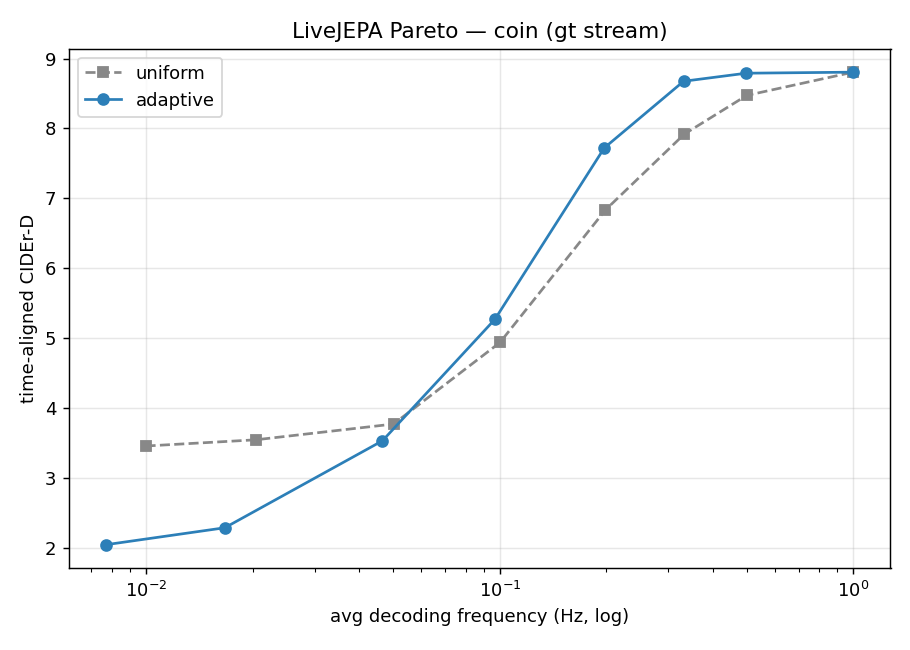
\includegraphics[width=0.86\linewidth]{figures/results_coin_gt.png}
\caption[COIN validation, ground-truth stream: adaptive vs uniform]{COIN validation, ground-truth stream (26 videos). Time-aligned CIDEr-D against decode rate for uniform and adaptive schedules. Adaptive holds CIDEr $\approx$ 7.7 at 0.20~Hz, a rate uniform does not reach until $\approx$ 0.31~Hz: $\approx 1.6\times$ fewer decoder invocations at equal quality. Below 0.10~Hz uniform recovers (Table~\ref{tab:coin-gt}).}
\label{fig:coin-gt}
\end{figure}

\begin{table}[htbp]
\centering\small
\caption{EgoExo4D validation keysteps, ground-truth stream (10 takes): time-aligned CIDEr-D by target decode rate.}
\label{tab:egoexo-keystep}
\begin{tabular}{rrr}
\toprule
\textbf{target Hz} & \textbf{uniform} & \textbf{adaptive} \\
\midrule
0.50 & 8.20 & 8.20 \\
0.35 & 8.12 & \textbf{8.20} \\
0.20 & 7.75 & \textbf{8.20} \\
0.10 & 6.54 & \textbf{7.38} \\
0.05 & \textbf{4.70} & 4.16 \\
0.02 & \textbf{2.37} & 1.58 \\
0.01 & \textbf{1.49} & 0.74 \\
\bottomrule
\end{tabular}
\end{table}

Adaptive holds the 8.20 plateau down to 0.20 Hz vs uniform's \textasciitilde{}0.50 Hz $\rightarrow$ \textbf{$\approx$2.5$\times$ fewer decodes} (Table~\ref{tab:egoexo-keystep}, Figure~\ref{fig:egoexo-keystep}). This is not directly comparable to the paper's 2.85$\times$, which is measured on atomic descriptions rather than keysteps (\S6.7--6.8). Both streams show a low-frequency \textbf{crossover} ($\leq$0.05 Hz), where uniform's even spacing wins --- so this is \emph{mid-band} dominance, not strict full-range Pareto dominance, whereas VL-JEPA reports adaptive ahead across its whole 0.01--2 Hz sweep. \textbf{Granularity finding:} on the raw EgoExo4D \emph{atomic}-description stream the same segmenter loses at every rate (\S6.7) --- adaptive placement needs temporally-stable meaning (\S6.8 asks what changes when the stream is predicted).

\begin{figure}[htbp]
\centering
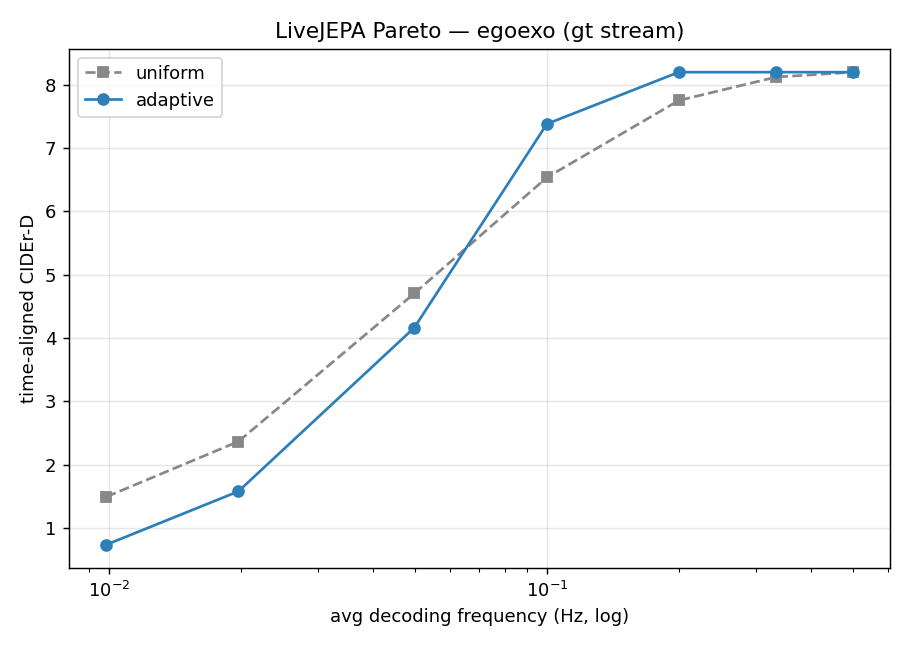
\includegraphics[width=0.86\linewidth]{figures/results_egoexo_keystep.png}
\caption[EgoExo4D keysteps, ground-truth stream: adaptive vs uniform]{EgoExo4D validation keysteps (10 takes), ground-truth stream. Adaptive holds the 8.20 plateau down to 0.20~Hz where uniform needs $\approx$ 0.50~Hz ($\approx 2.5\times$ fewer decodes; not comparable to the paper's $2.85\times$, which is measured on atomic descriptions). Note the crossover at $\leq$ 0.05~Hz, where uniform's even spacing wins: this is mid-band dominance, not strict full-range Pareto dominance.}
\label{fig:egoexo-keystep}
\end{figure}

\subsection{Online trigger correction}

At \textasciitilde{}0.10 Hz on EgoExo4D keysteps (Figure~\ref{fig:ablation-methods}): uniform 6.06, offline Ward 6.72, \textbf{naive online \textasciitilde{}3.5}, \textbf{corrected \texttt{SegmentTrigger} 7.2--7.7}. (This ablation harness scores the first 240 s of 6 keystep takes, so its absolute values differ from Table~\ref{tab:egoexo-keystep}.) The correction closes the gap between naive streaming and the offline oracle and even edges it out --- the real-time path works. (13/13 unit tests pass, including the trigger.)

\begin{figure}[htbp]
\centering
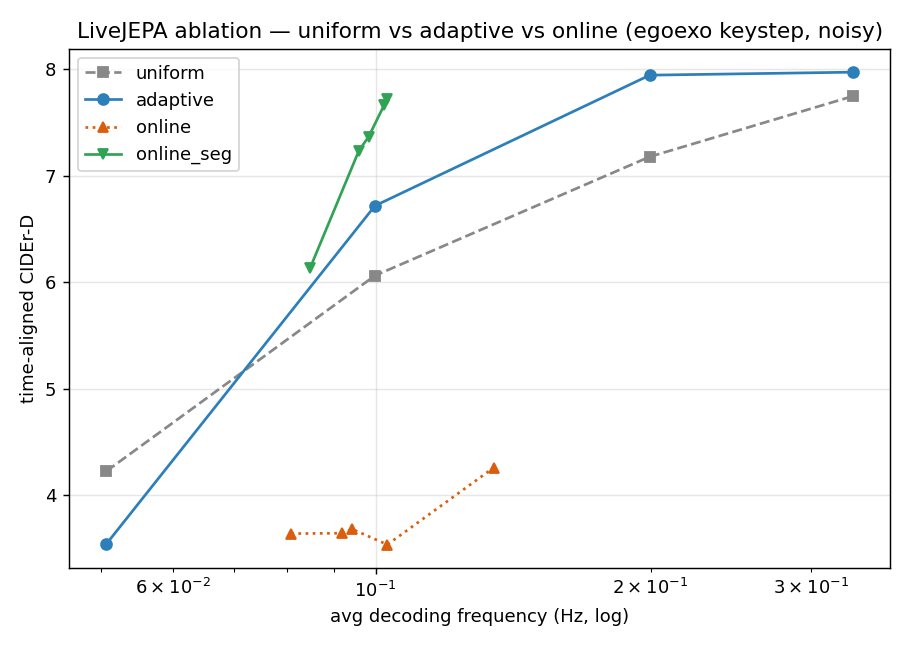
\includegraphics[width=0.86\linewidth]{figures/results_ablation_methods.png}
\caption[Method ablation on EgoExo4D keysteps at 0.10~Hz]{Method ablation at $\approx$ 0.10~Hz on EgoExo4D keysteps. The naive online trigger ($\approx 3.5$) falls well below uniform (6.06); the corrected \texttt{SegmentTrigger} (7.2--7.7) recovers the offline Ward result (6.72) and edges past it, which is what makes the real-time path viable.}
\label{fig:ablation-methods}
\end{figure}

\subsection{Full predicted pipeline}

\textbf{(a) Wide-predictor retrain --- the quality lever.} Retraining for 20k steps on class-diverse COIN (2962 train / 1118 val samples, \textasciitilde{}180 classes) gives held-out \textbf{cos(pred,target) = 0.636} on the 1118-sample diverse val, with \textbf{pred--pred cos = 0.504 (not collapsed)}. (On the two fixed validation sets of the later scaling study, \S6.5, the same checkpoint scores 0.667 and 0.772.) Captions capture the right action manifold with fuzzy object detail (e.g., "open the car key cover" $\rightarrow$ "open the back lid"; "stand up with straight legs" $\rightarrow$ exact). This lifted absolute end-to-end quality \textbf{$\approx$2.5$\times$} vs the earlier narrow predictor (below). \emph{This was the first rung of a larger data-scaling study, \S6.5.}

\textbf{(b) Predictor-in-the-loop Pareto --- 7 held-out COIN val videos} (Table~\ref{tab:coin-predictor}, Figure~\ref{fig:coin-predictor}).

\begin{table}[htbp]
\centering\small
\caption{Predictor-in-the-loop Pareto on 7 held-out COIN validation videos (2,962-clip predictor, no pre-smoothing): time-aligned CIDEr-D.}
\label{tab:coin-predictor}
\begin{tabular}{rrrl}
\toprule
\textbf{target Hz} & \textbf{uniform} & \textbf{adaptive} & \textbf{winner} \\
\midrule
1.00 & 2.611 & \textbf{2.814} & adaptive \\
0.50 & 2.644 & \textbf{2.779} & adaptive \\
0.35 & \textbf{2.856} & 2.735 & uniform \\
0.20 & \textbf{2.960} & 2.411 & uniform \\
0.10 & 2.124 & \textbf{2.415} & adaptive \\
0.05 & 2.191 & 2.150 & \textasciitilde{}tie \\
0.02 & 1.668 & 1.645 & \textasciitilde{}tie \\
0.01 & \textbf{1.960} & 0.977 & uniform \\
\bottomrule
\end{tabular}
\end{table}

Two things stand out. First, absolute CIDEr is now \textbf{2.6--3.0}, versus $\leq$1.2 for the pre-retrain narrow predictor --- the retrain, not the selective layer, drove that. Second, \textbf{adaptive no longer cleanly dominates}: it wins at high ($\geq$0.5 Hz) and sparse (0.1 Hz) rates, but \textbf{uniform peaks at 0.20 Hz (2.96)} and wins the mid-band. The reliable band is 0.2--1.0 Hz (n = 200--1000 decodes); the low-Hz tail (n = 10--53) is noise. N = 7 videos. These runs use no pre-smoothing (\texttt{smoothing\_window = 1}), the setting the sweep in (c) finds best. \S6.5 re-runs the same checkpoint on the same videos under the default \texttt{smoothing\_window = 3}, where adaptive's curve sits lower and it also loses at 0.5 Hz (2.561 vs 2.644).

\begin{figure}[htbp]
\centering
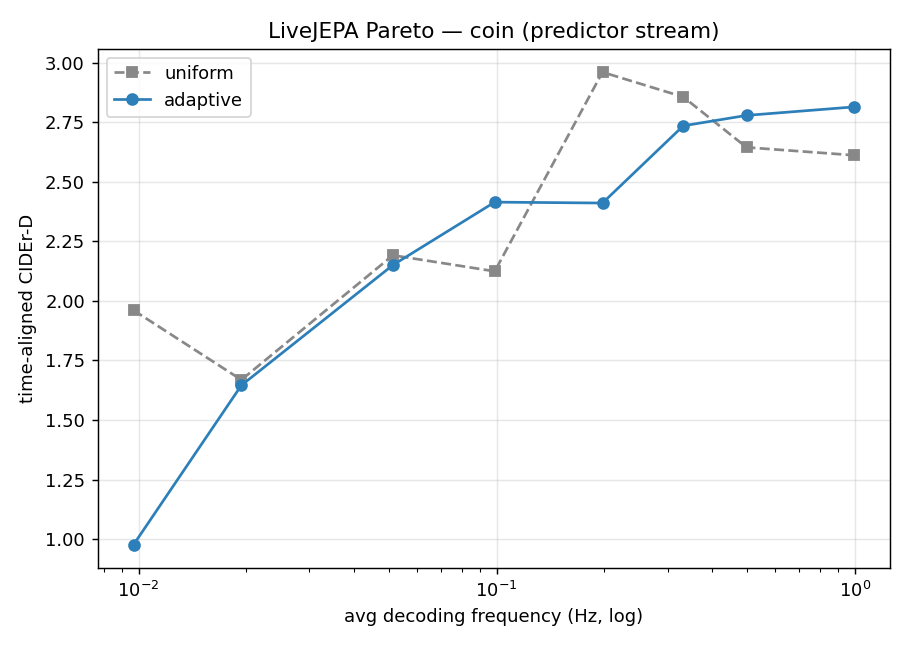
\includegraphics[width=0.86\linewidth]{figures/results_coin_predictor.png}
\caption[Predictor-in-the-loop Pareto on held-out COIN videos]{Predictor-in-the-loop Pareto on 7 held-out COIN validation videos (the full pipeline, no ground-truth stream). Adaptive wins at high ($\geq$ 0.5~Hz) and sparse (0.1~Hz) rates, but uniform peaks at 0.20~Hz and takes the mid-band -- the erosion of the mechanism's advantage as the upstream signal degrades.}
\label{fig:coin-predictor}
\end{figure}

\textbf{(c) Is the mid-band loss a tuning artifact? No.} We swept the segmenter's pre-smoothing window \texttt{smoothing\_window $\in$ \{1,3,5,7\}} (\S4.3) $\times$ \texttt{linkage $\in$ \{ward, average\}} on the cached streams, using the \emph{identical} SONAR decoder and CIDEr (the harness self-validates: the \texttt{smooth=1, ward} cell reproduces (b) to 3 decimals). \textbf{Every} smoothing setting made the mid-band \emph{worse}; the best config is the un-smoothed baseline (mean $\Delta$ = $-$0.061 vs uniform). At 0.20 Hz, uniform (2.96) beats \textbf{all eight} adaptive configurations. The attenuation is therefore \textbf{fundamental to predictor-stream noise}, not a mis-tuned trigger --- a clean negative result. The released configuration nevertheless keeps a 3-step window (\S4.3). On this COIN stream that slightly understates adaptive (\S6.5); on the EgoExo predicted stream it moves margins without changing a single winner (\S6.8).

\textbf{Interpretation.} On GT/keystep streams the segment structure is crisp, so adaptive places decodes exactly where meaning changes and wins. On the predicted stream the structure is fuzzy (predictor noise), so change-detection fires imperfectly; meanwhile 0.20 Hz $\approx$ one decode per 5 s $\approx$ the datasets' step cadence, where uniform's even spacing gives near-optimal coverage. The mechanism's advantage is real but \textbf{erodes as the upstream signal degrades}.

\subsection{Live demo (Phase 4)}

\texttt{demo.py} runs the full pipeline on webcam or video, decoding only when \texttt{SegmentTrigger} fires, with an annotated overlay (caption, a "DECODE" flash when the decoder actually runs, and a decodes/steps efficiency counter). It was verified end-to-end on real video; a bug was found and fixed where frames were sampled at native fps (near-duplicate windows) instead of subsampled to the working rate. On a COIN clip, adaptive decoded 2/40 windows (5\%) vs uniform 4/40 (10\%) --- \textbf{half the decodes} --- with sensible captions (e.g., "lift the barbell directly over the head"). A headless \texttt{--save-video} path renders the deliverable without a display.

The same pipeline is also packaged as a \textbf{web application}, serving the final COIN predictor of \S6.5. A FastAPI backend loads the models once and exposes REST endpoints plus two WebSocket streams, one for sample or uploaded video and one for webcam frames captured by the browser. The browser front end shows captions as they are emitted, a DECODE indicator, a timeline of decode events, a downloadable subtitle (.srt) file, and a live meter of the trigger's own signal --- the semantic shift 1 $-$ cos(newest embedding, recent-window centroid) --- against $\tau$, so a viewer can watch a caption fire at the moment the meter crosses the threshold. Uploads are validated, and the upload endpoint and both streams can be protected by an access token. The deployed server passed 15/15 end-to-end checks. Like the desktop demo, it runs slower than real time on the T1000 (\S8).

\subsection{Data-scaling study}

Because \S6.3 identified predictor caption quality (a \emph{data} property) as the limit on the full-system result, we scaled the predictor's training data while holding the architecture (29.9M params), the loss (InfoNCE + cosine) and both validation sets fixed. The first two rungs trained for 20k steps and the final one for 30k, so Table~\ref{tab:scaling} also reports the final run's 20k-step checkpoint, which separates data from training length. A three-lane extraction fleet (free Kaggle T4 + Colab + local T1000, working one shared video list) resolved \textbf{8,984 / 9,023 COIN training videos (99.6\%)} into a 26,360-clip feature cache.

\begin{table}[htbp]
\centering\small
\caption{Data scaling at fixed architecture: cosine to the SONAR target on the frozen 137-sample and diverse 956-sample validation sets, and mean pairwise cosine between predictions (pred--pred; lower is more diverse).}
\label{tab:scaling}
\begin{tabular}{rrrrr}
\toprule
\textbf{training clips} & \textbf{steps} & \textbf{frozen 137-val cos} & \textbf{diverse 956-val cos} & \textbf{pred--pred} \\
\midrule
2,962 & 20k & 0.772 & 0.667 & 0.527 \\
5,529 & 20k & 0.883 & 0.733 & 0.467 \\
26,360 & 20k & 0.882 & 0.832 & 0.394 \\
\textbf{26,360} & \textbf{30k} & \textbf{0.897} & \textbf{0.846} & \textbf{0.408} \\
\bottomrule
\end{tabular}
\end{table}

On the diverse 956-sample validation set (240 held-out videos) accuracy rose \textbf{+0.113 cos over the final 4.8$\times$ of data and had not saturated}. Most of that gain is data rather than training length: at a matched 20k steps the final data scale already reaches 0.832 (+0.099), and the extra 10k steps add +0.014. Predictions grew \emph{more} diverse (pred--pred 0.527 $\rightarrow$ 0.408), excluding collapse. The small frozen set saturates earlier: at matched length the last rung adds nothing there (0.883 $\rightarrow$ 0.882), and its final +0.015 comes from the extra steps. This isolates \textbf{data, not architecture or the selective layer, as the binding constraint} on caption quality, and motivates training on the paper's own data distribution (Action100M) as the next rung. It is also, to our knowledge, the first reported data-scaling curve for a VL-JEPA-style predictor.

Figure~\ref{fig:coin-scaling} repeats the predictor-in-the-loop evaluation of \S6.3(b) with the old and the final checkpoint on the same 7 videos. The final predictor roughly doubles absolute CIDEr in the 0.2--1.0 Hz band (4.9--5.4 against 2.4--3.0), yet the regime pattern is unchanged: adaptive wins at 1.0 and 0.1 Hz, and uniform holds the 0.2--0.5 Hz mid-band, coming closest at 0.35 Hz (5.07 vs 5.04). Both runs use the default \texttt{smoothing\_window = 3} (\S4.3), which is why the old checkpoint's adaptive curve here sits below Table~\ref{tab:coin-predictor}, which is un-smoothed.

\begin{figure}[htbp]
\centering
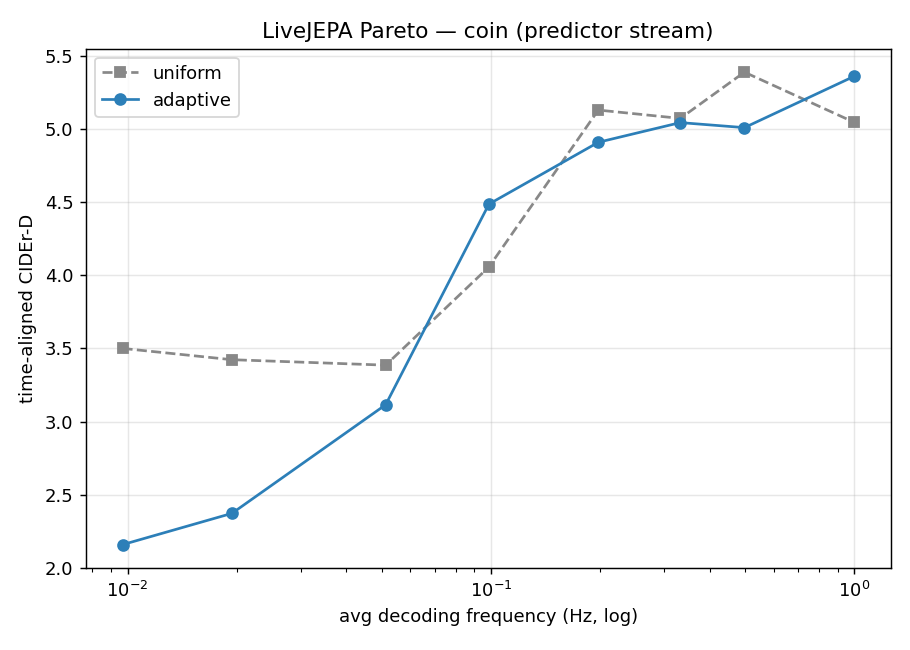
\includegraphics[width=0.48\linewidth]{figures/results_coin_predictor_c1final.png}
\hfill
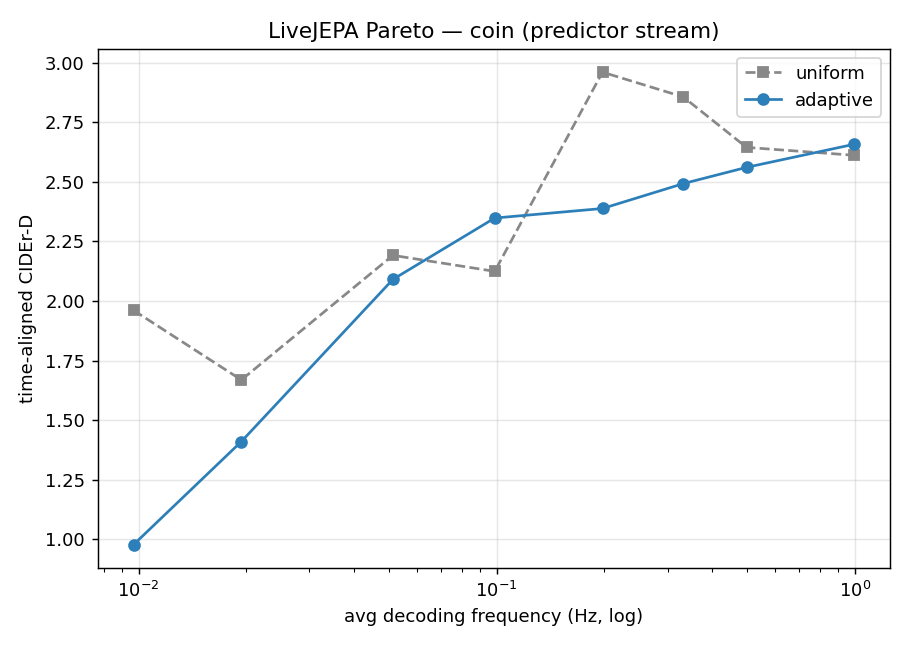
\includegraphics[width=0.48\linewidth]{figures/results_coin_predictor_c1old.png}
\caption[Full-system Pareto: final versus earlier COIN predictor]{Identical protocol, two predictors on the same 7 held-out COIN videos: the final 26{,}360-clip checkpoint (left) against the earlier 2{,}962-clip one (right), which score cos 0.846 and 0.667 on the same diverse validation set. The absolute lift comes from training data, not from the selective layer -- which is why the binding constraint is identified as data rather than architecture. Both panels use the default pre-smoothing (\texttt{smoothing\_window}~=~3), so the right panel's adaptive curve sits below the un-smoothed Table~\ref{tab:coin-predictor}.}
\label{fig:coin-scaling}
\end{figure}

\subsection{Training on the paper's own data (Action100M): a controlled negative}

VL-JEPA trains on \textbf{Action100M}~\cite{action100m2026}, whose captions are generated for HowTo100M~\cite{howto100m2019} videos; we trained on COIN step labels. To test whether that difference matters we rented an RTX 4090 (\textasciitilde{}\$8), extracted Action100M-preview features with a chunked download$\rightarrow$extract$\rightarrow$delete pipeline, and trained an otherwise identical predictor (20k steps, batch 64). YouTube rate-limiting capped extraction at \textbf{6,710 train / 160 val clips}, which --- fortuitously --- makes this a near-exact \emph{scale match} to our 5,529-clip COIN rung rather than a scale-up.

\begin{table}[htbp]
\centering\small
\caption{Predictor cosine to the SONAR target on three validation sets; C1-mid against C2 is the scale-matched control.}
\label{tab:a100m}
\begin{tabular}{p{0.42\linewidth}rrr}
\toprule
\textbf{model (training data)} & \textbf{COIN-137} & \textbf{COIN-956} & \textbf{A100M-160} \\
\midrule
C1-final (26,360 COIN, 30k steps) & \textbf{0.897} & \textbf{0.846} & 0.386 \\
C1-mid (5,529 COIN, 20k steps) & 0.883 & 0.733 & \textbf{0.401} \\
C2 (6,710 A100M, 20k steps) & 0.359 & 0.392 & 0.348 \\
\bottomrule
\end{tabular}
\end{table}

\textbf{Both COIN-trained models outperform the Action100M-trained model on Action100M's own validation set} (Table~\ref{tab:a100m}). The scale-matched control is decisive: C1-mid saw \emph{fewer} clips (5,529 vs 6,710) for the same 20k steps yet scores 0.401 vs 0.348, so the gap is not explained by training-set size.

Measuring the two corpora explains why, and the explanation is not the obvious one (Table~\ref{tab:vocab}):

\begin{table}[htbp]
\centering\small
\caption{Target-vocabulary statistics of the two training corpora.}
\label{tab:vocab}
\begin{tabular}{lrrr}
\toprule
\textbf{corpus} & \textbf{clips} & \textbf{unique captions} & \textbf{repeats per caption} \\
\midrule
COIN & 26,863 & 747 (3\%) & \textbf{36.0} \\
Action100M & 6,710 & 6,096 (91\%) & \textbf{1.1} \\
\bottomrule
\end{tabular}
\end{table}

COIN is effectively \textbf{closed-set}: 747 recurring step labels, each observed \textasciitilde{}36 times. Action100M is genuinely \textbf{open-vocabulary}: nearly every caption is unique and observed once. Inspection confirms A100M's captions are mostly sensible actions (\emph{"Sponging off powder from design surface"}, \emph{"puree the mixture in a blender"}), so this is not primarily a label-noise effect. The decoded outputs match the entropy explanation: C2 acquired the \emph{distribution of phrasings} but, with roughly one example per target, could not bind phrasing to content (\texttt{'Get a needle'} $\rightarrow$ \texttt{'Push the squeeze of the treats.'}), while the COIN models' closed vocabulary transfers out of domain as a coarse but useful prior.

\textbf{This qualifies our own headline.} The scaling result of \S6.5 is measured on a 747-label closed set, so a portion of the gain is improved closed-set discrimination rather than open-ended captioning ability. Cosine scores across the two corpora are therefore \textbf{not commensurable} --- they are different tasks sharing a metric. We report both rather than collapsing them.

\textbf{Augmentation does not rescue it either.} Replacing COIN with A100M loses; the natural remedy is to \emph{add} it. Training the identical recipe on the union (26,863 COIN + 6,710 A100M = 33,573 clips, the largest set in this work) gives COIN-137 \textbf{0.875}, COIN-956 \textbf{0.824}, A100M \textbf{0.390} --- slightly \emph{worse} on both COIN benchmarks than COIN alone (0.897, 0.846), and barely different on A100M (0.390 against 0.386 for the COIN-only model trained the same way, and below the smaller COIN rung's 0.401). The captions expose the mechanism: open-vocabulary targets contaminate previously exact closed-set outputs (\texttt{'squat and hold the barbell'} $\rightarrow$ \texttt{'sitbar and hold the barbell'}), and exact matches on the frozen benchmark fall from 7/10 to 5/10. A 25\% increase in data volume is outweighed by the entropy mismatch it introduces.

\textbf{Scope and the corrected lesson.} This evaluates the 10\% \emph{preview} release at \textasciitilde{}6.7k clips; VL-JEPA used the full 1.2M-video corpus, where an open vocabulary is adequately covered. The defensible claim is narrow but useful: \emph{open- vocabulary supervision requires orders of magnitude more data than closed-set supervision to reach comparable predictive accuracy} --- so a low-resource reconstruction is better served by a small closed-vocabulary corpus, and the apparent "win" of a closed set partly reflects an easier task.

\subsection{Paper-protocol EgoExo4D --- atomic descriptions at scale (the boundary)}

We finally ran the paper's headline benchmark: EgoExo4D validation, \textbf{atomic action descriptions}, time-aligned CIDEr-D over a frequency sweep, on the \textbf{218 density-matched validation takes} (annotation counts closest to the paper's \textasciitilde{}143/video; our pool runs sparser at median 100). This is the density regime the paper's 2.85$\times$ headline is quoted on.

\begin{table}[htbp]
\centering\small
\caption{EgoExo4D atomic descriptions, 218 density-matched validation takes, ground-truth stream: time-aligned CIDEr-D by target decode rate.}
\label{tab:egoexo-atomic}
\begin{tabular}{rrr}
\toprule
\textbf{target Hz} & \textbf{uniform} & \textbf{adaptive} \\
\midrule
1.00 & \textbf{4.48} & 3.57 \\
0.50 & \textbf{3.47} & 3.11 \\
0.35 & \textbf{2.91} & 2.79 \\
0.20 & \textbf{2.31} & 2.26 \\
0.10 & \textbf{1.78} & 1.60 \\
0.05 & \textbf{1.40} & 1.21 \\
0.02 & \textbf{1.08} & 0.89 \\
0.01 & \textbf{0.91} & 0.76 \\
\bottomrule
\end{tabular}
\end{table}

\textbf{Uniform wins at every frequency} (Table~\ref{tab:egoexo-atomic}, Figure~\ref{fig:egoexo-atomic}) --- there is no iso-quality speedup for adaptive on atomic descriptions. Far from contradicting the mechanism, this \textbf{completes} the picture from \S6.1: keysteps (\textasciitilde{}1 event / 15 s) are redundant and adaptive wins \textasciitilde{}2.5$\times$; atomic descriptions (\textasciitilde{}1 event / 2 s) are saturated with change and adaptive loses. The benefit tracks temporal redundancy monotonically. The gap to the paper's positive atomic result is instructive and honest: our measurement is a clean \textbf{gt-mode} stream that isolates the segmenter on raw annotation density, whereas the paper's number comes from their \emph{predicted} (denoised) stream. Whether a predicted stream recovers an advantage at atomic density --- and whether any such advantage comes from placement or from averaging --- is the question \S6.8 answers; the result here is its baseline.

\begin{figure}[htbp]
\centering
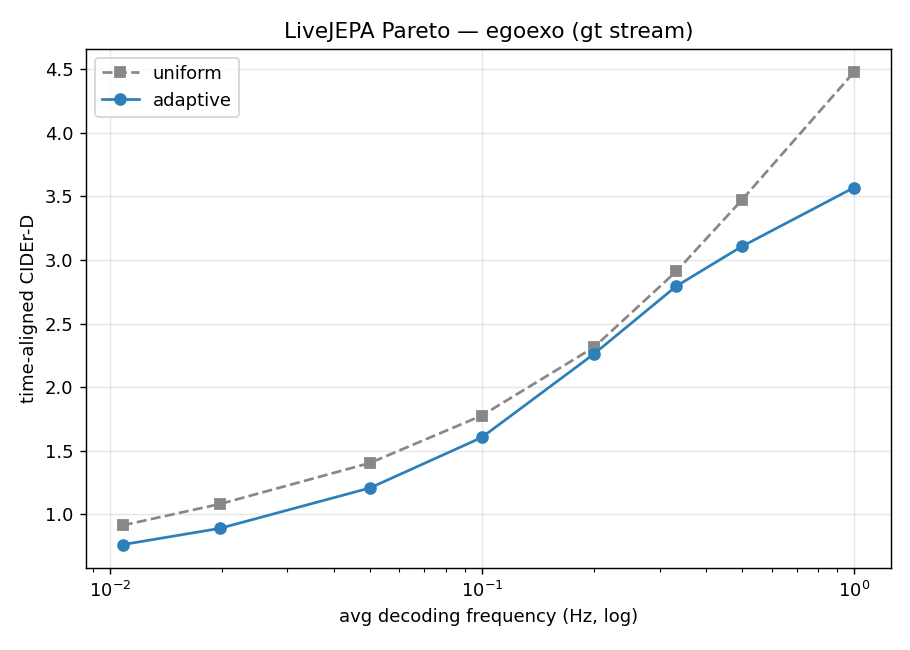
\includegraphics[width=0.86\linewidth]{figures/results_egoexo_atomic_218.png}
\caption[EgoExo4D atomic descriptions, ground-truth stream (218 takes)]{EgoExo4D atomic descriptions on 218 density-matched validation takes, ground-truth stream. \textbf{Uniform wins at every frequency.} At $\approx$ 1 event / 2~s the stream is saturated with change and offers nothing to segment -- the redundancy boundary of the mechanism. Figure~\ref{fig:egoexo-indomain} shows the same benchmark on the predicted stream.}
\label{fig:egoexo-atomic}
\end{figure}

\medskip

\subsection{The predicted stream: averaging, not placement}

\S6.7 evaluated atomic descriptions on a \emph{clean} ground-truth stream and found uniform superior at every budget. VL-JEPA's headline, however, was measured on their \textbf{predicted} stream. Testing that required a predictor able to caption EgoExo: our COIN-trained model produced semantically correct but stylistically alien output ("remove the chain" against annotations phrased "the camera wearer takes a tire lever from the table with his right hand"), collapsing CIDEr to \textbf{0.012 for both methods} --- an unmeasurable comparison rather than a result.

We therefore trained an in-domain predictor on 11,556 (window, caption) pairs from 627 EgoExo validation takes, windowed identically to inference, for 20k steps. (Extraction stopped at its 12,000-sample cap, gating pairs included, before the 721-take candidate pool was exhausted.) The 40 evaluation takes were excluded from training and 25 further takes were held out for gating (cos \textbf{0.599}, pred--pred 0.325). The exclusion is by take: evaluation takes share participants and, for 39 of 40, recording sessions with training takes (\S8).

\textbf{Three schedules, not two.} Adaptive decodes the \emph{mean} of each segment of a pre-smoothed stream; plain uniform decodes a single stream step. VL-JEPA reports that average pooling gives consistent gains for both schedules, so its uniform baseline pools too. We therefore score three schedules at every budget --- uniform, adaptive, and uniform+pool, which decodes the mean of a fixed block of the same smoothed stream at uniform's own timestamps (\S4.3) --- and, as a reference with no timing at all, a single decode per take of its whole stream's mean.

\begin{table}[htbp]
\centering\small
\caption{Headline benchmark. EgoExo4D atomic descriptions, 40 held-out takes, predicted stream from the in-domain predictor: time-aligned CIDEr-D for each schedule at each decode budget (best of the three in bold).}
\label{tab:egoexo-indomain}
\begin{tabular}{rrrrr}
\toprule
\textbf{avg Hz} & \textbf{decodes} & \textbf{uniform} & \textbf{adaptive} & \textbf{uniform+pool} \\
\midrule
0.998 & 7072 & 0.296 & 0.330 & \textbf{0.335} \\
0.499 & 3537 & 0.310 & \textbf{0.348} & 0.342 \\
0.333 & 2357 & 0.299 & 0.340 & \textbf{0.358} \\
0.199 & 1412 & 0.287 & 0.333 & \textbf{0.341} \\
0.100 & 706 & 0.282 & 0.331 & \textbf{0.338} \\
0.050 & 357 & 0.278 & \textbf{0.338} & 0.319 \\
0.020 & 140 & 0.249 & 0.312 & \textbf{0.314} \\
0.011 & 76 & 0.305 & 0.302 & \textbf{0.322} \\
\bottomrule
\end{tabular}
\end{table}

\textbf{Against plain uniform, adaptive wins 7 of 8 budgets} (Table~\ref{tab:egoexo-indomain}, Figure~\ref{fig:egoexo-indomain}), losing only the degenerate 0.011 Hz point (\textasciitilde{}2 decodes per take), and absolute quality rises \textbf{25$\times$} (0.012 $\rightarrow$ 0.33) from training in-domain. Plain uniform's CIDEr barely depends on rate: it stays between 0.278 and 0.310 at every budget except 0.02 Hz (0.249). Anchored on its best score anywhere (0.310 at 3537 decodes), adaptive matches it at 0.050 Hz with 357 decodes --- $\approx$9.9$\times$ fewer decoder invocations, the figure an earlier version of this thesis quoted as its headline.

\textbf{That comparison confounds placement with averaging.} Uniform+pool scores above plain uniform at every budget, by 5--26\%, and once pooling is matched adaptive's advantage disappears: uniform+pool is higher at six of eight budgets, and its best score (0.358 at 2357 decodes) exceeds adaptive's best anywhere (0.348), so no efficiency multiple can be quoted against it. Per take (\S6.9) the two are statistically tied at six budgets; adaptive is significantly better at 0.05 Hz and significantly worse at 0.35 Hz. On the semantic metric uniform+pool is ahead at all eight. What the predicted stream rewards is averaging its noise before decoding --- and fixed blocks average it as well as Ward segments do.

\textbf{The benchmark rewards a good summary more than good timing.} One decode per take --- the mean of its whole stream, 40 decodes for the whole set --- scores CIDEr 0.284, about what plain uniform reaches with 1412 decodes (0.287 at 0.2 Hz). EgoExo takes are internally repetitive (mean pairwise caption similarity 0.669), so a representative caption matches many annotations wherever it is placed. This bounds how much any placement policy can show on this protocol, ours and the paper's alike.

\begin{figure}[htbp]
\centering
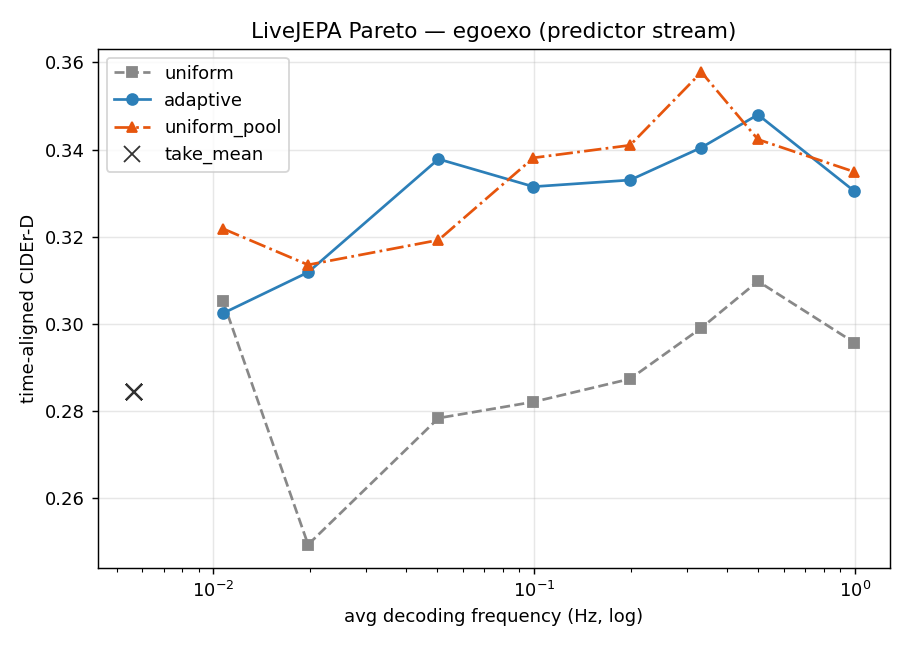
\includegraphics[width=0.86\linewidth]{figures/results_egoexo_predictor_40_indomain_pooled.png}
\caption[Headline: three schedules on the predicted stream]{\textbf{Headline result.} The atomic-description benchmark of Figure~\ref{fig:egoexo-atomic}, on 40 of its takes, with the stream \emph{predicted} by an in-domain predictor. Adaptive (blue) beats uniform decoding of single points (grey) at 7 of 8 budgets, but uniform with the same pooling (orange) matches it, scoring higher at 6 of 8. The cross is one decode per take of the whole stream's mean (40 decodes in all), which scores about as well as plain uniform at 0.2~Hz.}
\label{fig:egoexo-indomain}
\end{figure}

\textbf{Why the original controls missed this.} Three controls had been designed against an earlier, out-of-domain artifact (Figure~\ref{fig:egoexo-rejected}) and were repeated here, and each compared adaptive with an \emph{unpooled} baseline. (i) The semantic metric's lift over a shuffled alignment rises from +0.0012 out of domain to \textbf{+0.0225--0.0284} in domain, so the metric does register timing; that finding stands. (ii) With mean-pooling disabled, adaptive kept a flat +0.031--0.040 advantage over uniform at every budget, which we had read as temporal selection isolated from averaging. But disabling pooling left the 3-step pre-smoothing (\S4.3) on the adaptive stream alone, so each "exact" adaptive point was still a three-step average. Given the same smoothing, uniform points score within 0.003 of adaptive's at every budget: the flat margin was the smoothing (Figure~\ref{fig:egoexo-indomain-controls}). (iii) Adaptive beat random placement at 8 of 8 budgets, but the random points were unpooled as well. Removing the pre-smoothing altogether does not rescue placement either: adaptive then trails uniform+pool on the semantic metric at all eight budgets, by 0.009--0.016.

Against plain uniform, the result does not depend on the pre-smoothing. With it disabled, adaptive still leads uniform at all eight budgets on the semantic metric, by +0.013 at 1 Hz rising to +0.102 at 0.02 Hz, and on CIDEr it wins the same seven budgets and again loses only the 0.011 Hz point. The cell behind the 9.9$\times$ figure is unchanged (0.338 at 357 decodes), while at the two highest rates the margin narrows from about +0.035 to about +0.010.

\begin{figure}[htbp]
\centering
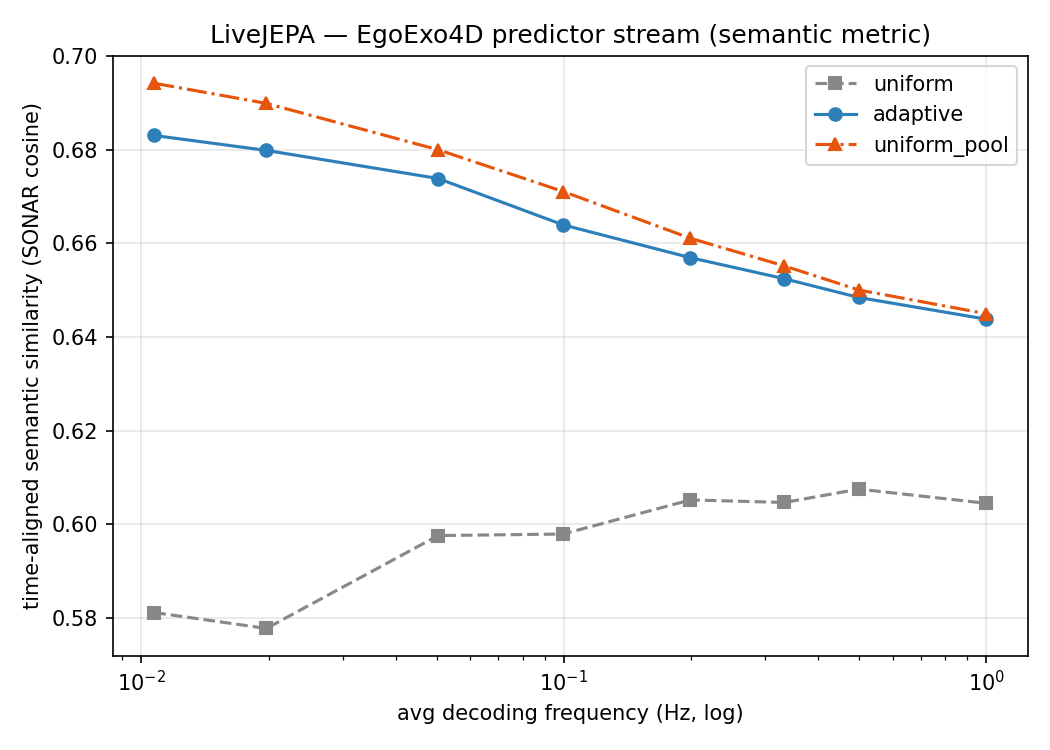
\includegraphics[width=0.48\linewidth]{figures/results_egoexo_predictor_40_indomain_semantic_pooled.png}
\hfill
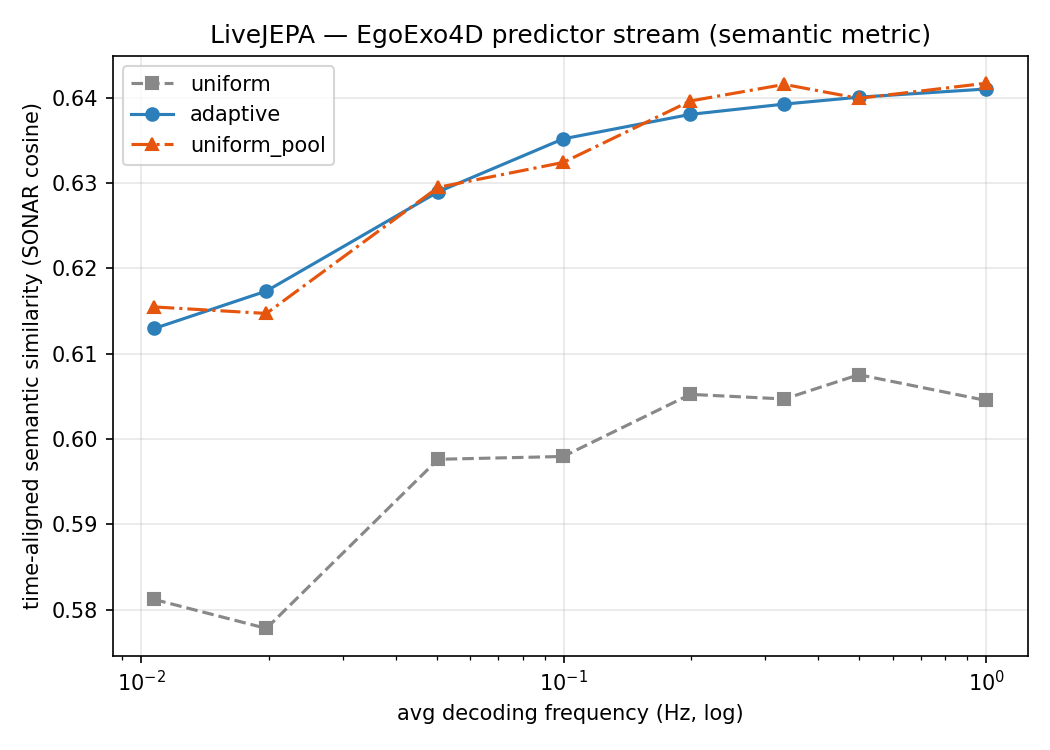
\includegraphics[width=0.48\linewidth]{figures/results_egoexo_predictor_40_indomain_semantic_nopool_pooled.png}
\caption[Controls: the semantic metric with a matched baseline]{Controls on the semantic metric, same takes. Left: with pooling, uniform+pool (orange) sits just above adaptive at every budget. Right: with mean-pooling disabled but the 3-step pre-smoothing still applied, adaptive's flat lead over plain uniform (grey) vanishes against uniform points given the same smoothing (orange) -- the margin once read as temporal selection was the smoothing.}
\label{fig:egoexo-indomain-controls}
\end{figure}

\textbf{Interpretation.} The reversal from \S6.7 is real but narrower than it first looked. On exactly these 40 takes the ground-truth stream favours uniform at 7 of 8 budgets --- adaptive edges it only at 0.20 Hz (2.38 vs 2.35) --- whereas on the predicted stream adaptive beats plain uniform at 7 of 8. The stream is the only difference, and what changes is not that the predicted stream offers plateaus to segment but that it is \emph{noisy}: averaging that noise before decoding is worth 5--26\% CIDEr, and fixed blocks capture it as well as Ward segments do. VL-JEPA reports both that pooling helps both schedules and that adaptive selection Pareto-dominates uniform across its sweep; in our reconstruction the first replicates and the second does not. We do not claim this transfers to VL-JEPA itself: its predictor (490M parameters, trained on Action100M) and embedding space differ from ours, and a predictor with crisper semantic structure could restore a placement advantage at matched pooling (\S8).

\begin{figure}[htbp]
\centering
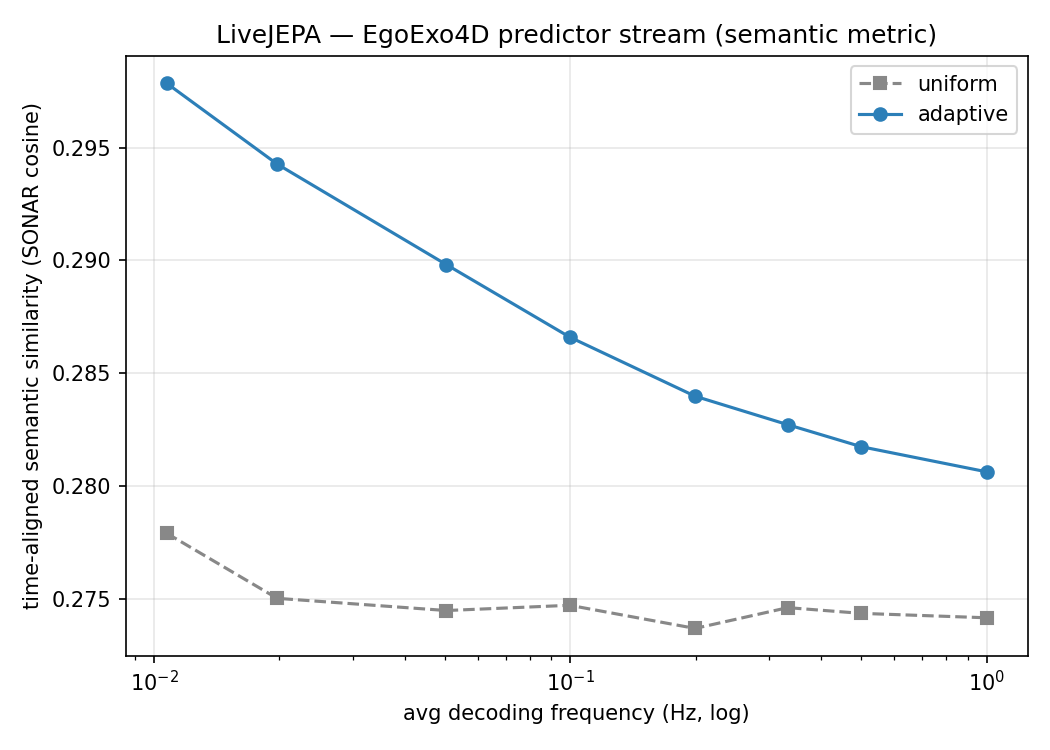
\includegraphics[width=0.48\linewidth]{figures/results_egoexo_predictor_40_semantic.png}
\hfill
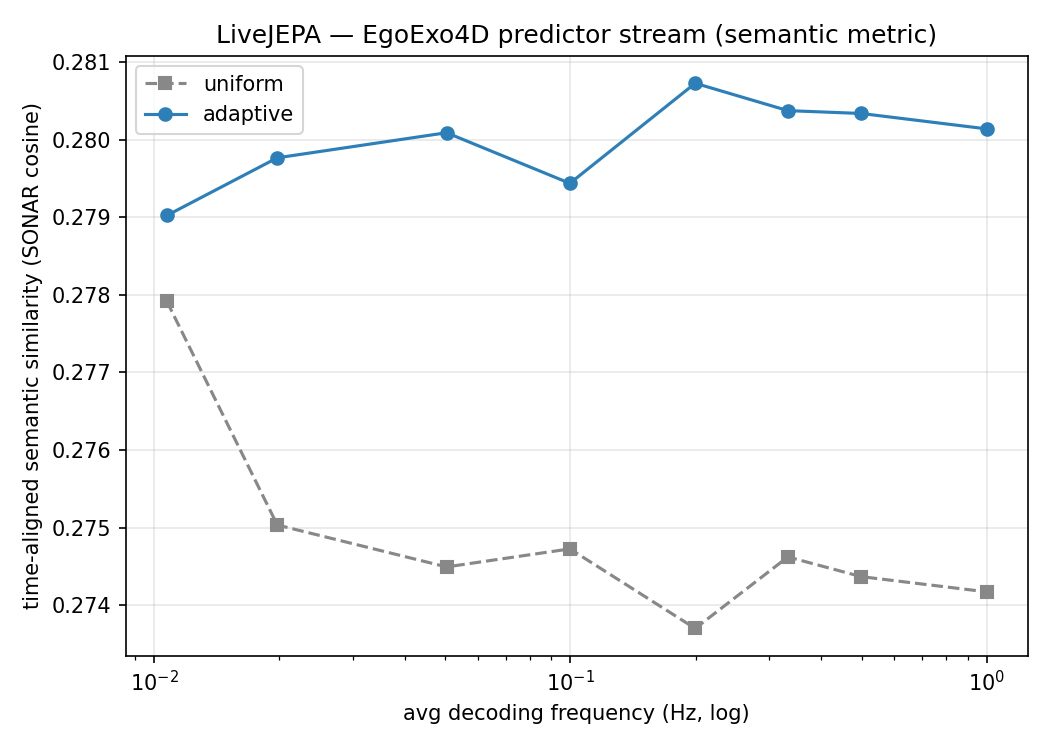
\includegraphics[width=0.48\linewidth]{figures/results_egoexo_predictor_40_semantic_nopool.png}
\caption[The rejected out-of-domain result and its pooling ablation]{The rejected artifact, retained because the original controls were defined against it. An out-of-domain predictor appeared to show adaptive winning 8/8 on the semantic metric (left), but with pooling disabled the advantage collapses (right): the effect was denoising, not selection. The in-domain run's apparent survival of the same check rested on pre-smoothing applied to adaptive alone (Figure~\ref{fig:egoexo-indomain-controls}).}
\label{fig:egoexo-rejected}
\end{figure}

\subsection{Significance, and what the headroom analysis can show}

Two questions a reader will put to \S6.8: \emph{are the margins real across only 40 videos}, and \emph{how close to optimal is any trigger?}

\textbf{Significance.} We score every take separately and bootstrap the \textbf{paired} difference between adaptive and each baseline over 5,000 resamples; pairing is the correct design because the schedules see the identical take, so take-difficulty variance cancels (Table~\ref{tab:paired}, Figure~\ref{fig:egoexo-rigor}).

\begin{table}[htbp]
\centering
\caption[Paired per-take differences against both baselines]{Paired per-take differences, adaptive minus each baseline, over 40 held-out takes and 5,000 bootstrap resamples. Bold: the 95\% interval excludes zero. In brackets: takes favouring adaptive, of 40.}
\label{tab:paired}
\small
\begin{tabular}{rcccc}
\toprule
& \multicolumn{2}{c}{\textbf{vs uniform}} & \multicolumn{2}{c}{\textbf{vs uniform+pool}} \\
\cmidrule(lr){2-3}\cmidrule(lr){4-5}
\textbf{target Hz} & \textbf{semantic} & \textbf{CIDEr} & \textbf{semantic} & \textbf{CIDEr} \\
\midrule
1.00 & \textbf{+0.0397} (40) & \textbf{+0.0193} (26) & \textbf{$-$0.0013} (12) & $-$0.0055 (21) \\
0.50 & \textbf{+0.0419} (40) & \textbf{+0.0212} (26) & \textbf{$-$0.0017} (12) & $-$0.0004 (24) \\
0.35 & \textbf{+0.0484} (40) & \textbf{+0.0255} (28) & \textbf{$-$0.0027} (7) & \textbf{$-$0.0113} (11) \\
0.20 & \textbf{+0.0523} (40) & \textbf{+0.0263} (23) & \textbf{$-$0.0043} (3) & $-$0.0026 (15) \\
0.10 & \textbf{+0.0675} (40) & \textbf{+0.0300} (28) & \textbf{$-$0.0070} (2) & $-$0.0062 (21) \\
0.05 & \textbf{+0.0776} (39) & \textbf{+0.0279} (27) & \textbf{$-$0.0066} (5) & \textbf{+0.0143} (29) \\
0.02 & \textbf{+0.1057} (40) & \textbf{+0.0365} (27) & \textbf{$-$0.0099} (5) & $-$0.0035 (13) \\
0.01 & \textbf{+0.1057} (40) & $-$0.0017 (19) & \textbf{$-$0.0111} (1) & $-$0.0076 (9) \\
\bottomrule
\end{tabular}
\end{table}

Against plain uniform the semantic margin is significant at all eight budgets, with 40/40 takes favouring adaptive at seven of them, and per-take CIDEr favours adaptive at seven budgets, significantly at all seven; at the degenerate 0.011 Hz point the difference is null ($-$0.002, 95\% CI [$-$0.037, +0.031], 19/40 takes). Against uniform+pool the semantic metric reverses --- uniform+pool is significantly ahead at all eight budgets --- and on CIDEr the two are tied at six, with adaptive significantly ahead at 0.05 Hz (+0.014, [+0.006, +0.023], 29/40 takes) and significantly behind at 0.35 Hz ($-$0.011, [$-$0.020, $-$0.002], 11/40). One significant cell each way among eight is what no consistent effect looks like. CIDEr has visibly lower statistical power than the semantic metric --- n-gram overlap over \textasciitilde{}100 events is high-variance, whereas cosine similarity is smooth.

\begin{figure}[htbp]
\centering
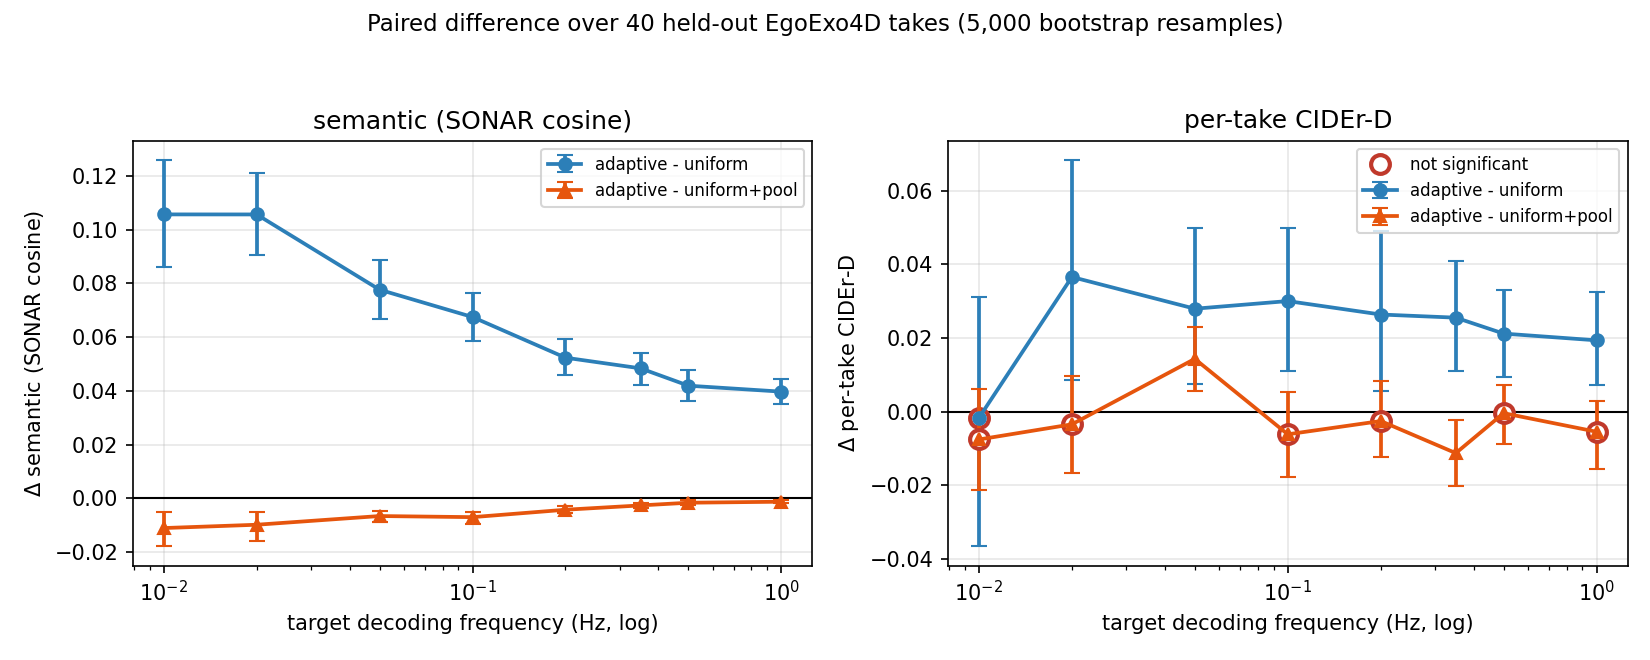
\includegraphics[width=0.86\linewidth]{figures/results_egoexo_rigor.png}
\caption[Paired bootstrap of adaptive against both baselines over 40 takes]{Paired bootstrap over 5{,}000 resamples: the per-take difference between adaptive and each baseline, with 95\% confidence intervals. Against uniform decoding of single points (blue) adaptive is ahead on both metrics. Against uniform with the same pooling (orange) the semantic difference is negative at every budget and the CIDEr difference straddles zero. Non-significant cells are circled.}
\label{fig:egoexo-rigor}
\end{figure}

\textbf{Headroom.} We then asked how close a schedule comes to the best score the semantic metric allows. The \emph{best-window ceiling} takes, for each annotation, the maximum over all contiguous ranges of cos(mean(stream[a:b]), gt). Uniform and dense decoding use single points of the stream, the whole-take reference uses the mean of one range, and the pooled schedules use span means of the stream they segment --- which, under the default pre-smoothing (\S4.3), is the smoothed stream. The same ceiling computed on the smoothed stream is lower (0.7661), and the per-annotation maximum over both streams is 0.7721, within 0.0001 of the raw-stream figure in Table~\ref{tab:ceiling}; so that figure upper-bounds every row of the table (Figure~\ref{fig:egoexo-ceiling}).

\begin{table}[htbp]
\centering\small
\caption{Headroom on the semantic metric (40 held-out takes, 95\% bootstrap intervals): each reference as a percentage of the best-window ceiling.}
\label{tab:ceiling}
\begin{tabular}{p{0.42\linewidth}lr}
\toprule
\textbf{reference} & \textbf{score (95\% CI)} & \textbf{\% of ceiling} \\
\midrule
uniform @0.05 Hz & 0.5949 [0.5740, 0.6167] & 77.1\% \\
dense --- decode \textbf{every} timestep, no selection & 0.6037 [0.5854, 0.6243] & 78.2\% \\
GT-boundary --- segment the \emph{ground-truth caption} stream & 0.6684 [0.6522, 0.6851] & 86.6\% \\
adaptive @0.05 Hz & 0.6725 [0.6560, 0.6898] & 87.1\% \\
uniform+pool @0.05 Hz & 0.6791 [0.6626, 0.6963] & 88.0\% \\
one decode per take --- the whole stream's mean & 0.6950 [0.6791, 0.7117] & 90.0\% \\
best-frame ceiling & 0.7541 [0.7396, 0.7692] & 97.7\% \\
\textbf{best-window ceiling} (upper bound) & \textbf{0.7720} [0.7577, 0.7867] & 100\% \\
\bottomrule
\end{tabular}
\end{table}

\begin{figure}[htbp]
\centering
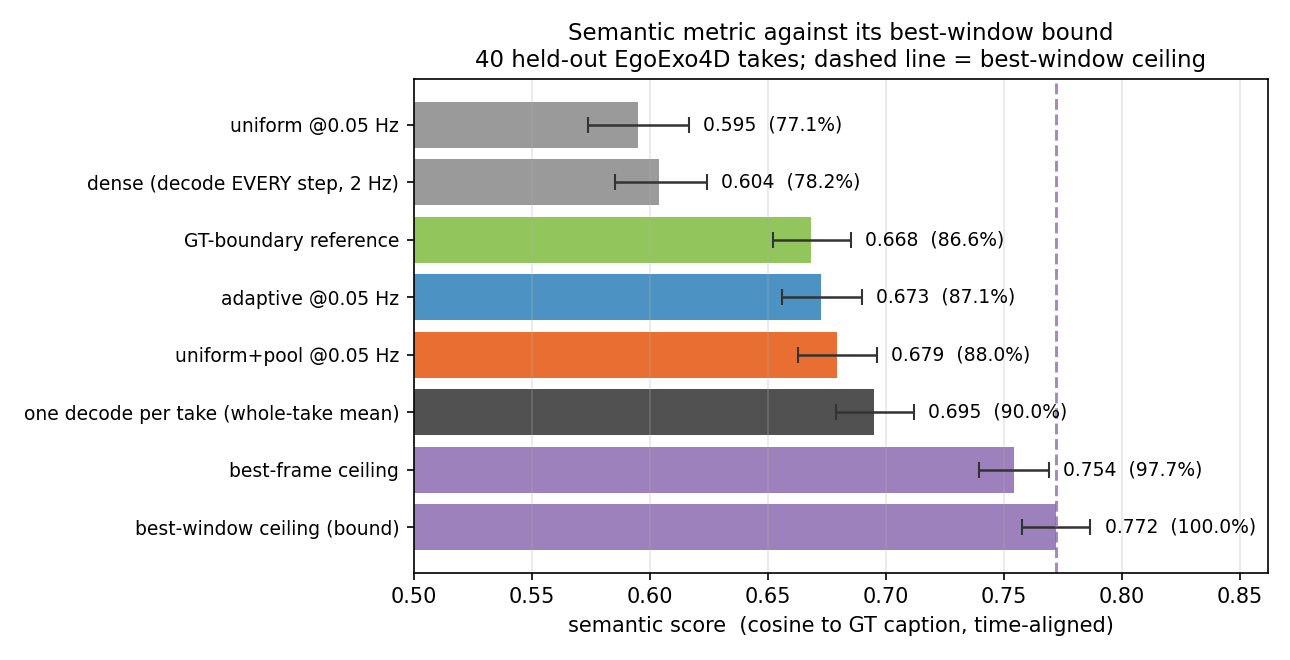
\includegraphics[width=0.86\linewidth]{figures/results_egoexo_ceiling.png}
\caption[The semantic metric against its best-window bound]{The semantic metric against its best-window bound, an upper bound on any method that decodes a point or a pooled mean of a contiguous span (with pre-smoothing taken into account the bound moves by 0.0001; see text). Every pooled schedule beats decoding every frame, whichever boundaries it uses, and a single whole-take mean, with no timing at all, scores highest of all -- so the bound measures how well pooled summaries match captions, not how good a trigger is.}
\label{fig:egoexo-ceiling}
\end{figure}

Three findings follow; the third corrects an earlier reading.

\emph{Pooling beats decoding more.} Single-point decoding is flat in rate --- uniform scores 0.5949 at 0.05 Hz, 0.6054 at 0.5 Hz, and 0.6037 decoding every timestep --- while every pooled schedule exceeds decode-everything at a small fraction of its cost. On a noisy predicted stream, averaging before decoding is not merely cheaper; it is better. The +0.018 gap between the best-window and best-\emph{frame} ceilings says the same: a pooled span carries signal no individual timestep does.

\emph{Where the boundaries fall barely matters.} Ward boundaries (0.6725), the annotators' own boundaries (0.6684) and fixed blocks (0.6791) land within 0.011 of one another. Annotation boundaries are homogeneous in caption space and Ward's in predictor space, but on this stream neither beats a fixed grid.

\emph{The bound cannot rank triggers here.} An earlier version of this thesis read adaptive's 87.1\% as a near-exhausted trigger and placed the remaining headroom in the predictor. A policy with no trigger at all --- one mean per take --- reaches 90.0\%, above every adaptive budget, because EgoExo takes are repetitive enough that a take-level summary sits close to most of their captions. The semantic metric therefore rewards averaging in itself: it can compare schedules at matched pooling, as in Table~\ref{tab:paired}, but it cannot certify a trigger as near-optimal.

\emph{Provenance note.} Our first implementation of the boundary oracle returned a score \textbf{below uniform}, which is impossible for an upper bound and was a code fault rather than a result: the ground-truth stream is timestamped from t = 0 while the predicted stream carries window-centre times beginning \textasciitilde{}3.75 s in, so index-based mapping misaligned every decode by \textasciitilde{}4 s, and the oracle compared exact embeddings against adaptive's pooled ones. Both were corrected before the numbers above were produced. We record it because the diagnostic generalises: an upper bound that loses to the method it bounds is a bug, not a finding.

\section{Discussion}

The headline lesson is about \textbf{where an idealized mechanism meets reality}, and it arrives in three parts that must be read together.

\textbf{On clean streams, placement decides quality, and pays only where the stream is redundant.} On ground-truth COIN steps and EgoExo keysteps, adaptive placement beats uniform across the mid-band (\S6.1); on the raw atomic-annotation stream, saturated with an event every two seconds, it loses at every budget, over the 218-take pool and at 7 of 8 budgets on the 40 takes of \S6.8 (\S6.7--6.8). The value of placing decodes adaptively tracks the redundancy of the stream it reads.

\textbf{On a predicted stream, averaging decides quality, and fixed intervals capture it.} Against uniform decoding of single points, adaptive wins 7 of 8 budgets on the predicted stream over the same 40 atomic takes where the annotation stream favours uniform (\S6.8). But the predicted stream differs from the annotation stream by being noisy, and what adaptive brings to it is pooling: given the same pooling, uniform decoding matches adaptive on CIDEr and beats it on the semantic metric. VL-JEPA reports that pooling helps both schedules and that adaptive selection still Pareto-dominates uniform; in our reconstruction the first half replicates and the second does not. On COIN's predicted stream, where adaptive was compared with \emph{plain} uniform and still lost the mid-band (0.2--0.35 Hz without pre-smoothing, 0.2--0.5 Hz with it; \S6.3, \S6.5), the same reading applies with more force, since 0.2 Hz $\approx$ COIN's intrinsic step cadence and even spacing already matches the true event rate there.

\textbf{What limits caption quality is the predictor.} We had argued this from the ceiling analysis, which turned out not to support it (\S6.9); the evidence that remains is more direct. Replacing a COIN-trained predictor with an in-domain one raised CIDEr 25$\times$ on the same takes (\S6.8); scaling COIN data 9$\times$ raised held-out accuracy from cos 0.667 to 0.846 with the curve still climbing (\S6.5); and on the predicted stream the choice between adaptive and fixed-interval spans made no consistent difference. Pooling, under either schedule, also beats decoding every frame at a fraction of the cost (\S6.9): on a noisy predicted stream it is a way to get a \textbf{better} answer, not only a cheaper one.

This clarifies what is a \emph{predictor} problem versus a \emph{mechanism} problem. Caption correctness (vocabulary, object detail) is a predictor/data-scale property; the selective policy decides \emph{when} to decode, not \emph{what}. Separating these two axes is, we think, the most transferable result here --- and \S6.6's entropy analysis sharpens it further, showing that what looked like a domain-match question was really a question about the entropy of the target vocabulary.

\textbf{A methodological note.} Four times in this project a positive result did not survive its own controls, and saying so is part of the contribution. An earlier out-of-domain semantic win proved to be denoising rather than selection (\S6.8). A "noisy labels" explanation for the Action100M negative was contradicted by measurement and replaced by the entropy account (\S6.6). An upper bound that lost to the method it bounded turned out to be a time-alignment bug, and when the corrected version \emph{still} did not exceed adaptive, the right conclusion was that the label "oracle" was wrong, not the number (\S6.9). And the headline of an earlier version of this thesis --- adaptive's 7-of-8 win on the predicted stream, which had survived three controls --- did not survive a fourth: giving the uniform baseline the pooling the paper gives it. The control meant to rule averaging out had left the pre-smoothing on one side only. The lesson generalises: a control is only as good as the match between its two arms, and every difference between them other than the hypothesis is a confound until it is removed.

\medskip

\section{Limitations}

\begin{itemize}
\item \textbf{Small COIN predicted-stream eval (N = 7 videos).} The \S6.3/\S6.5 conclusions rest on 7 held-out videos; the low-frequency tail is explicitly noise. Uniform's 0.20 Hz peak is robust to trigger tuning but not to sample size. (The EgoExo predicted-stream results, \S6.8--6.9, are on 40 takes with per-take CIs and do not share this weakness.)
\item \textbf{The EgoExo predicted-stream comparison is 40 takes, not 218.} \S6.8 uses 40 held-out takes; the frozen 218-take pool exists and the same protocol would run on it, at \textasciitilde{}84 h on the local T1000. The paired bootstrap separates the schedules where they differ; more takes would tighten the ties between adaptive and uniform+pool.
\item \textbf{Evaluation takes are disjoint from training by take, not by person or session.} All 40 evaluation takes share a participant and a physical setting with training takes, and 39 of 40 share a recording session. All schedules consume the same predicted stream, so the comparison between them is internally fair, but absolute quality --- including the 25$\times$ rise over the COIN-trained predictor --- partly reflects familiarity with those people and places. A participant-disjoint retrain needs no new extraction (it keeps 483 takes / 8,822 pairs, 76\% of the training data) and is the most useful next control (\S9).
\item \textbf{The non-replication is specific to our reconstruction.} Our predictor (29.9M parameters, in-domain) and embedding space (SONAR) differ from VL-JEPA's (490M parameters, trained on Action100M, its own learned space), and EgoExo takes are internally repetitive (caption self-similarity 0.669), which favours averaging over timing. A predictor with crisper semantic structure might restore a placement advantage at matched pooling. The paper also does not specify the window over which its uniform baseline pools; ours --- a block of one decode interval around each decode point --- is one reasonable choice, not the only one.
\item \textbf{One pre-smoothing setting throughout.} Results from \S6.5 onward use the configuration's 3-step moving average, which was never tuned on EgoExo; on COIN the sweep of \S6.3 found no smoothing marginally better. On the EgoExo predicted stream, disabling it narrows adaptive's high-rate margin over plain uniform without removing it, and leaves uniform+pool ahead of adaptive on the semantic metric at every budget (\S6.8).
\item \textbf{The semantic metric rewards averaging.} A single whole-take mean scores above every adaptive budget (\S6.9), so the metric can compare schedules at matched pooling but cannot certify a trigger as near-optimal, and its best-window ceiling measures how well pooled summaries match captions rather than trigger quality.
\item \textbf{The benchmark is weakly sensitive to timing.} One caption per take scores CIDEr 0.284 against 0.287 for uniform decoding at 0.2 Hz (\S6.8). Any comparison of triggers on this protocol, the paper's included, has little room to show a difference in placement.
\item \textbf{Different embedding space.} SONAR (chosen for invertibility) is not VL-JEPA's space, so absolute CIDEr is not comparable --- only the relationships between schedules are.
\item \textbf{Two predictors, two vocabularies.} The COIN predictor is trained on \textasciitilde{}180 closed-set classes; the EgoExo predictor on 11.5k in-domain pairs. Neither is open-domain, and \S6.6 shows why that gap is a data-scale problem: open-vocabulary targets at \textasciitilde{}1 example each are not learnable at our budget.
\item \textbf{Action100M conclusions are scoped to the preview release} (\textasciitilde{}6.7k clips after throttling), not the full 1.2M-video corpus VL-JEPA used.
\item \textbf{CIDEr has low statistical power at these scales} (\S6.9: 23--28/40 takes vs 40/40 on the semantic metric against plain uniform); we report both metrics for this reason, and the semantic metric is ours, not the paper's.
\item \textbf{Not real-time on the test hardware.} V-JEPA 2 is \textasciitilde{}11 s/window on a T1000.
\item \textbf{Granularity dependence.} Adaptive placement requires temporally-stable meaning: it fails on very dense \emph{annotation} streams, and on our predicted stream it does no better than fixed-interval pooling.
\end{itemize}

\medskip

\section{Conclusion and Future Work}

We reconstructed VL-JEPA's selective-decoding mechanism from released components, corrected its online realization, and stress-tested it against its own claims.

Selective decoding \textbf{beats uniform across the mid-band on temporally redundant streams} ($\approx$1.6$\times$ on COIN steps, $\approx$2.5$\times$ on EgoExo4D keysteps), with uniform recovering at the lowest rates, and on the paper's own atomic-description benchmark it \textbf{loses at every budget when the stream is raw annotation}. On the predicted stream it beats uniform decoding of single points at 7 of 8 budgets, significantly on both metrics --- but that gain is \textbf{averaging}. Given the same pooling, which the paper's protocol gives both schedules, uniform decoding matches adaptive (tied at six of eight budgets, one significant win each way) and reaches a higher best score. In our reconstruction, then, the paper's adaptive-over-uniform result holds on clean redundant streams but does not replicate like for like on a predicted one, where what pays is averaging the predictor's noise before decoding, under any schedule. That the benchmark scores one caption per video about as well as uniform decoding at 0.2 Hz is a caution for any work that compares triggers on it. A data-scaling study on the full COIN split (cos 0.667 $\rightarrow$ \textbf{0.846}, still climbing) and the 25$\times$ gain from in-domain training show that the predictor is the lever for caption quality, while two controlled negatives on Action100M show that lever is a question of target-vocabulary entropy rather than domain match. The project is a working, reproducible system with a defensible --- and, where the evidence demanded it, negative --- scientific story.

\textbf{Future work,} ordered by what the evidence above actually recommends. (1) \textbf{Predictor capacity and in-domain data}, the lever for caption quality (\S6.5, \S6.8); \S6.6 predicts the route is \textasciitilde{}10--100$\times$ more open-vocabulary data (free via Kaggle), not a different mixing strategy. (2) \textbf{An evaluation that rewards timing.} Time-aligned CIDEr on EgoExo atomic descriptions scores a single caption per take like a 0.2 Hz schedule; scoring only annotations that differ from their take's typical content, or reporting every schedule against that one-caption reference, would let placement show whatever value it has. (3) \textbf{Retrain the in-domain predictor participant-disjoint} from the evaluation takes (\S8) --- no new extraction is needed --- to confirm the absolute numbers without shared people and sessions. (4) \textbf{Scale the predicted-stream comparison from 40 to 218 takes} on the frozen pool, tightening the ties between adaptive and uniform+pool. (5) A \textbf{hybrid policy} --- a pooled uniform floor plus extra decodes on detected change --- as the most plausible way for placement to add to pooling, and to recover COIN's mid-band. (6) A \textbf{pretrained-VLM variant}: the trigger is decoder-agnostic, so pairing it with a strong pretrained captioner would give open-domain accuracy while keeping decode-on-change efficiency. (7) The optional \textbf{LiveCC token-generative baseline}~\cite{livecc2025} for a like-for-like comparison. (8) \textbf{Real-time deployment}: the web application of \S6.4 already streams captions, but slower than real time on the T1000; faster hardware is the remaining step.

\medskip

\appendix
\section{Reproducibility}

Set \texttt{project.use\_stubs: false} in \texttt{configs/default.yaml}; models cache in \texttt{\textasciitilde{}/.cache/huggingface/hub}. Key commands (full list in \texttt{RESULTS.md}):

Two checkpoints are referenced throughout: \texttt{checkpoints\_c1\_final/predictor\_30000.pt} (the COIN model, cos 0.846, also the deployed one) and \texttt{checkpoints\_egoexo/predictor\_20000.pt} (the in-domain EgoExo model used for \S6.8--6.9 only). Earlier sections were measured on \texttt{checkpoints\_kaggle/predictor\_20000.pt} (cos 0.636 on the older 1,118-sample validation set; 0.667 and 0.772 on the fixed sets of \S6.5); that is noted where it matters, and \S6.5 reports both.

Two details matter for exact reproduction. First, \texttt{configs/default.yaml} sets \texttt{selective.smoothing\_window: 3}, the setting behind every adaptive result from \S6.5 onward; set it to 1 to reproduce \S6.3(b). Second, the diverse validation directory \texttt{data\_cache\_coin\_full\_val} has since gained 21 late clips from the same held-out videos (977 files now). The \S6.5 figures use the 956 that predate them, so the evaluation command below now prints 0.844 rather than 0.846 for the final checkpoint.

\begin{lstlisting}
# Mechanism (clean GT streams)                                          -> 6.1
python -m livejepa.run_eval --dataset coin --mode gt
python -m livejepa.run_eval --dataset egoexo --mode gt --gt-source keystep --max-videos 10 --max-seconds 300
# Ablations + tests                                                     -> 6.2
python scripts/ablations.py
python -m pytest tests/ -q                      # 16/16
# Predictor quality, data-scaling rungs                                 -> 6.5
python scripts/eval_predictor.py --ckpt checkpoints_c1_final/predictor_30000.pt --val data_cache_coin2_val --decode
python scripts/eval_predictor.py --ckpt checkpoints_c1_final/predictor_30000.pt --val data_cache_coin_full_val
python scripts/eval_predictor.py --ckpt checkpoints_c1_final/predictor_20000.pt --val data_cache_coin_full_val  # matched steps
# Full predicted-pipeline Pareto + tuning sweep                         -> 6.5, 6.3
python -m livejepa.run_eval --dataset coin --mode predictor --ckpt checkpoints_c1_final/predictor_30000.pt --coin-split val --max-videos 7 --max-seconds 180
python scripts/tune_adaptive.py --ckpt checkpoints_kaggle/predictor_20000.pt
# Action100M rungs C2 / C3                                              -> 6.6
python scripts/eval_predictor.py --ckpt checkpoints_c2/predictor_20000.pt --val data_cache_a100m_val --decode
python -m livejepa.train --config configs/default.yaml --data-root "data_cache_coin_full,data_cache_a100m" \
    --ckpt-dir checkpoints_c3_combined --max-steps 30000 --batch-size 32
# Atomic descriptions, clean GT stream (the negative)                   -> 6.7
python -m livejepa.run_eval --dataset egoexo --mode gt --gt-source atomic \
    --uids-file eval_data/egoexo_takes_218.txt --max-seconds 360 --out results_egoexo_atomic_218
# In-domain predictor: build cache, train, then the three-schedule Pareto -> 6.8
python scripts/build_egoexo_cache.py --max-per-take 20 --max-samples 12000 \
    --exclude-uids eval_data/egoexo_takes_pred40.txt
python -m livejepa.train --config configs/default.yaml --data-root data_cache_egoexo \
    --ckpt-dir checkpoints_egoexo --max-steps 20000 --batch-size 32
python -m livejepa.run_eval --dataset egoexo --mode predictor --gt-source atomic \
    --ckpt checkpoints_egoexo/predictor_20000.pt \
    --uids-file eval_data/egoexo_takes_pred40.txt --max-seconds 360 \
    --methods uniform,adaptive,uniform_pool,take_mean \
    --decode-cache eval_data/decode_cache_egoexo_indomain.jsonl \
    --out results_egoexo_predictor_40_indomain_pooled
python scripts/eval_semantic_pareto.py --ckpt checkpoints_egoexo/predictor_20000.pt \
    --uids-file eval_data/egoexo_takes_pred40.txt --max-seconds 360 \
    --methods uniform,adaptive,random,uniform_pool --out <name>   # + --pool none
# Significance, headroom, figures                                       -> 6.9
python scripts/eval_rigor.py   --ckpt checkpoints_egoexo/predictor_20000.pt \
    --uids-file eval_data/egoexo_takes_pred40.txt --max-seconds 360 \
    --methods uniform,adaptive,uniform_pool,take_mean --boot 5000 \
    --out results_egoexo_rigor_pooled
python scripts/eval_ceiling.py --ckpt checkpoints_egoexo/predictor_20000.pt \
    --uids-file eval_data/egoexo_takes_pred40.txt --max-seconds 360
python scripts/make_thesis_figures.py --rigor results_egoexo_rigor_pooled.json
# Live demo (headless annotated MP4)                                    -> 6.4
python -m livejepa.demo --source <video.mp4> --ckpt checkpoints_c1_final/predictor_30000.pt \
    --no-display --save-video demo_adaptive.mp4 --mode adaptive
\end{lstlisting}

\section{Figures and artifacts}

Every figure listed here is placed inline in the section named beside it; Table~\ref{tab:figure-map} is the index, not the figures themselves. All are collected in \texttt{thesis\_materials/figures/}, catalogued by \texttt{thesis\_materials/INDEX.md}; every \texttt{.png} ships with the \texttt{.json} it was plotted from, and \texttt{thesis\_materials/TABLES.md} holds every table in this chapter. The two \texttt{.mp4} demo recordings cannot be embedded in a PDF and are referenced by name only.

\begin{table}[htbp]
\centering\small
\caption{Where each figure and demo artifact appears.}
\label{tab:figure-map}
\begin{tabular}{lp{0.42\linewidth}}
\toprule
\textbf{\S} & \textbf{Figures} \\
\midrule
6.1 & \texttt{results\_coin\_gt.png}, \texttt{results\_egoexo\_keystep.png} \\
6.2 & \texttt{results\_ablation\_methods.png} \\
6.3 & \texttt{results\_coin\_predictor.png} (predictor-in-the-loop Pareto), \texttt{results\_adaptive\_tuning.json} (tuning sweep, table only) \\
6.4 & \texttt{demo\_adaptive.mp4}, \texttt{demo\_uniform.mp4} \\
6.5 & \texttt{results\_coin\_predictor\_c1final.png}, \texttt{results\_coin\_predictor\_c1old.png} \\
6.7 & \texttt{results\_egoexo\_atomic\_218.png} \\
6.8 & \texttt{results\_egoexo\_predictor\_40\_indomain\_pooled.png} \textbf{(headline, three schedules)}, \texttt{results\_egoexo\_predictor\_40\_indomain\_semantic\_pooled.png}, \texttt{results\_egoexo\_predictor\_40\_indomain\_semantic\_nopool\_pooled.png}; the rejected out-of-domain run, \texttt{results\_egoexo\_predictor\_40\_semantic.png} and \texttt{results\_egoexo\_predictor\_40\_semantic\_nopool.png}. The two-schedule versions of the earlier draft (\texttt{results\_egoexo\_predictor\_40\_indomain*.png} without \texttt{\_pooled}) are kept for provenance \\
6.9 & \texttt{results\_egoexo\_rigor.png} (paired CIs against both baselines), \texttt{results\_egoexo\_ceiling.png} (headroom) \\
\bottomrule
\end{tabular}
\end{table}
